% =========================================================================
%  DESIGN MANUAL — Mountain Climber Health & GPS Tracker
% =========================================================================
\documentclass[12pt, a4paper, openany]{report}

% ── Load Shared Preamble ──
% =========================================================================
%  Shared LaTeX Preamble — Mountain Climber Health & GPS Tracker
%  Used by both User Manual and Design Manual
% =========================================================================

\usepackage[utf8]{inputenc}
\usepackage[T1]{fontenc}
\usepackage{lmodern}

% ── Page Geometry ──
\usepackage[a4paper, margin=2.5cm, top=3cm, bottom=3cm]{geometry}

% ── Colors ──
\usepackage{xcolor}
\definecolor{teal600}{HTML}{0D9488}
\definecolor{teal700}{HTML}{0F766E}
\definecolor{teal100}{HTML}{CCFBF1}
\definecolor{slate800}{HTML}{1E293B}
\definecolor{slate600}{HTML}{475569}
\definecolor{slate400}{HTML}{94A3B8}
\definecolor{amber500}{HTML}{F59E0B}
\definecolor{red500}{HTML}{EF4444}
\definecolor{blue500}{HTML}{3B82F6}
\definecolor{green600}{HTML}{16A34A}
\definecolor{chaptergray}{HTML}{F1F5F9}

% ── Typography ──
\usepackage{titlesec}
\usepackage{titletoc}

\titleformat{\chapter}[display]
  {\normalfont\huge\bfseries\color{slate800}}
  {\chaptertitlename\ \thechapter}{20pt}{\Huge}
\titleformat{\section}
  {\normalfont\Large\bfseries\color{teal700}}{}{0em}{\thesection\quad}
\titleformat{\subsection}
  {\normalfont\large\bfseries\color{slate800}}{}{0em}{\thesubsection\quad}
\titleformat{\subsubsection}
  {\normalfont\normalsize\bfseries\color{slate600}}{}{0em}{\thesubsubsection\quad}

% ── Headers & Footers ──
\usepackage{fancyhdr}
\pagestyle{fancy}
\fancyhf{}
\fancyhead[L]{\small\color{slate400}\leftmark}
\fancyhead[R]{\small\color{slate400}\rightmark}
\fancyfoot[C]{\small\color{slate400}\thepage}
\renewcommand{\headrulewidth}{0.4pt}
\renewcommand{\footrulewidth}{0pt}

% ── Graphics & Figures ──
\usepackage{graphicx}
\usepackage{float}
\usepackage{wrapfig}
\usepackage{subcaption}
\graphicspath{{figures/}{../shared/figures/}}

% ── Tables ──
\usepackage{booktabs}
\usepackage{tabularx}
\usepackage{longtable}
\usepackage{colortbl}
\usepackage{multirow}
\newcommand{\tablemark}{\rowcolor{chaptergray}}

% ── Code Listings ──
\usepackage{listings}
\lstset{
  basicstyle=\small\ttfamily,
  backgroundcolor=\color{chaptergray},
  frame=single,
  rulecolor=\color{slate400},
  keywordstyle=\color{teal700}\bfseries,
  commentstyle=\color{slate400}\itshape,
  stringstyle=\color{amber500},
  breaklines=true,
  numbers=left,
  numberstyle=\tiny\color{slate400},
  numbersep=8pt,
  tabsize=2,
  showstringspaces=false
}

% ── TikZ for Diagrams ──
\usepackage{tikz}
\usetikzlibrary{arrows.meta, positioning, shapes.geometric, fit, calc, backgrounds, decorations.markings, decorations.pathreplacing}

% ── Callout Boxes ──
\usepackage[most]{tcolorbox}

\newtcolorbox{infobox}[1][]{
  colback=teal100!30,
  colframe=teal600,
  coltitle=white,
  fonttitle=\bfseries,
  title={\textcolor{white}{ℹ\quad Info}},
  #1
}

\newtcolorbox{warningbox}[1][]{
  colback=amber500!10,
  colframe=amber500,
  coltitle=white,
  fonttitle=\bfseries,
  title={\textcolor{white}{⚠\quad Warning}},
  #1
}

\newtcolorbox{cautionbox}[1][]{
  colback=red500!10,
  colframe=red500,
  coltitle=white,
  fonttitle=\bfseries,
  title={\textcolor{white}{⛔\quad Caution}},
  #1
}

\newtcolorbox{tipbox}[1][]{
  colback=green600!10,
  colframe=green600,
  coltitle=white,
  fonttitle=\bfseries,
  title={\textcolor{white}{💡\quad Tip}},
  #1
}

% ── Hyperlinks & Cross-references ──
\usepackage[colorlinks=true, linkcolor=teal700, urlcolor=blue500, citecolor=teal600]{hyperref}
\usepackage{bookmark}

% ── Misc ──
\usepackage{enumitem}
\usepackage{pdfpages}
\usepackage{amsmath}

% ── Image Placeholder Command ──
\newcommand{\imagePlaceholder}[3][0.8\textwidth]{%
  \begin{figure}[H]
    \centering
    \fcolorbox{slate400}{chaptergray}{%
      \parbox{#1}{%
        \vspace{2cm}
        \centering
        \textcolor{slate400}{\large\textbf{[ IMAGE PLACEHOLDER ]}}\\[6pt]
        \textcolor{slate600}{\texttt{\detokenize{#2}}}
        \vspace{2cm}
      }%
    }
    \caption{#3}
    \label{fig:#2}
  \end{figure}
}

% =========================================================================
%  Title Page Template — Mountain Climber Health & GPS Tracker
%  Arguments: #1 = Document Title, #2 = Document Subtitle
% =========================================================================

\newcommand{\maketitlepage}[2]{
  \begin{titlepage}
    \centering
    
    \vspace*{1cm}
    
    % ── Logos ──
    \begin{minipage}{0.35\textwidth}
      \centering
      
\includegraphics[height=2.5cm]{uop-logo.png}
    \end{minipage}
    \hfill
    \begin{minipage}{0.35\textwidth}
      \centering
      
\includegraphics[height=2.5cm]{product-logo.png}
    \end{minipage}
    
    \vspace{1.5cm}
    
    % ── University & Department ──
    {\large\textcolor{slate600}{University of Peradeniya}}\\[4pt]
    {\normalsize\textcolor{slate400}{Faculty of Engineering}}\\[2pt]
    {\normalsize\textcolor{slate400}{Department of Computer Engineering}}
    
    \vspace{1.5cm}
    
    % ── Title ──
    \rule{\textwidth}{1.5pt}\\[12pt]
    {\Huge\bfseries\textcolor{slate800}{#1}}\\[12pt]
    {\Large\textcolor{teal700}{#2}}\\[12pt]
    \rule{\textwidth}{1.5pt}
    
    \vspace{1.5cm}
    
    % ── Project ──
    {\large\textcolor{slate600}{Mountain Climber Health \& GPS Tracker}}\\[6pt]
    {\normalsize\textcolor{slate400}{Third Year Design Project (3YP)}}\\[4pt]
    {\normalsize\textcolor{slate400}{Group 23}}
    
    \vspace{1.5cm}
    
    % ── Team Members ──
    \begin{minipage}{0.8\textwidth}
      \centering
      {\normalsize\textbf{Team Members}}\\[10pt]
      \begin{tabular}{l l}
        \textcolor{slate600}{Sahan Jayasundara}  & \textcolor{slate400}{E/21/198} \\[4pt]
        \textcolor{slate600}{Prabash Rathnayaka}  & \textcolor{slate400}{E/21/328} \\[4pt]
        \textcolor{slate600}{Pasan Sandeep}       & \textcolor{slate400}{E/21/353} \\
      \end{tabular}
    \end{minipage}
    
    \vspace{1cm}
    
    % ── Supervisors ──
    \begin{minipage}{0.8\textwidth}
      \centering
      {\normalsize\textbf{Academic Supervisors}}\\[10pt]
      \begin{tabular}{l}
        \textcolor{slate600}{Dr. Isuru Nawinne} \\[4pt]
        \textcolor{slate600}{Ms. Yashodha Vimukthi} \\
      \end{tabular}
    \end{minipage}
    
    \vfill
    
    % ── Date ──
    {\normalsize\textcolor{slate400}{September 2026}}
    
  \end{titlepage}
}


\begin{document}

% ── Title Page ──
\maketitlepage{Design Manual}{System Architecture \& Engineering Specification}

% ── Table of Contents ──
\tableofcontents
\clearpage

% ── List of Figures & Tables ──
\listoffigures
\listoftables
\clearpage

% ── Chapters ──
\chapter{Introduction}
\label{ch:introduction}

\section{Project Motivation}
Mountaineering and high-altitude hiking are physically demanding activities fraught with environmental hazards. Every year, numerous accidents and fatalities occur due to unpredictable weather, sudden health complications such as Acute Mountain Sickness (AMS), and getting lost in remote terrains. A critical factor exacerbating these situations is the lack of reliable, off-grid communication. Conventional cellular networks are typically unavailable in mountainous regions, meaning that when an emergency strikes, climbers cannot promptly call for help. This results in significantly delayed search-and-rescue (SAR) operations, drastically reducing the chances of survival for the victims. The Mountain Climber Health and GPS Tracker project was conceived to address this critical gap by providing a robust, standalone communication and health monitoring system that operates independently of traditional infrastructure.

\section{Problem Statement}
The core problem addressed by this project is the inability to reliably monitor the vital signs of mountaineers and track their geographical locations in areas devoid of cellular coverage. When a climber faces distress—whether due to physical injury, cardiac issues, or spatial disorientation—there is currently no reliable method for them to automatically alert their base camp or fellow climbers. The lack of an integrated system that combines real-time health telemetry, continuous GPS tracking, and decentralized long-range communication severely hampers the effectiveness and timeliness of emergency response in alpine environments.

\section{Project Objectives}
To address the aforementioned challenges, this project aims to achieve the following specific objectives:
\begin{itemize}
    \item \textbf{Real-Time Health Monitoring:} Continuously measure and record critical vital signs, including heart rate and blood oxygen saturation (SpO$_2$), using a wearable device to detect early signs of physiological distress.
    \item \textbf{Continuous GPS Tracking:} Accurately track the climber's geographical coordinates in real-time, allowing base camp operators to monitor their exact location and movement trajectory.
    \item \textbf{Off-Grid LoRa Mesh Communication:} Establish a reliable, low-power, long-range communication network using LoRa technology, configured in a mesh topology to overcome the line-of-sight limitations typical of mountainous terrains.
    \item \textbf{Automated Distress Signaling:} Implement an automated SOS alert mechanism that triggers immediately if a climber's vital signs fall outside safe thresholds or if they manually initiate a panic sequence.
    \item \textbf{Cross-Platform Visualization:} Develop intuitive user interfaces, including a mobile application for climbers and a comprehensive desktop dashboard for base camp operators, to visualize data and facilitate communication.
\end{itemize}

\section{Project Scope}
\subsection{Inclusions}
The scope of this project encompasses the design, development, and integration of both hardware and software components. This includes:
\begin{itemize}
    \item The design and fabrication of the Climber Main Device, Wristband, Repeater nodes, and Base Camp Unit using ESP32 microcontrollers.
    \item Implementation of a custom LoRa communication protocol utilizing SX1278 transceivers at 433 MHz.
    \item Development of a BLE communication link between the Wristband and the user's smartphone.
    \item Development of a cross-platform mobile application using Flutter/Dart for local monitoring and messaging.
    \item Creation of a Python Flask-based local dashboard for the base camp, featuring real-time maps and health data visualization.
    \item A web portal built with Next.js and Supabase for device registration and e-commerce functionalities related to mountaineering gear.
\end{itemize}

\subsection{Exclusions}
The following aspects are explicitly excluded from the current scope of the project:
\begin{itemize}
    \item Integration with global satellite communication networks (e.g., Iridium or Inmarsat).
    \item Clinical certification of the health monitoring sensors; the devices are intended for informational and preliminary warning purposes, not as certified medical equipment.
    \item Mass production and commercial packaging of the hardware devices.
\end{itemize}

\section{Document Structure Overview}
This design manual is organized to provide a comprehensive understanding of the system's architecture and engineering details:
\begin{itemize}
    \item \textbf{Chapter 2: System Architecture} details the overall structural design, data flow, and deployment strategy of the system.
    \item \textbf{Chapter 3: Hardware Design} provides an in-depth look at the electronic components, circuit designs, and power management for each physical device.
    \item \textbf{Chapter 4: Communication Protocols} explains the proprietary data formats and communication standards implemented across LoRa, BLE, WiFi, and Serial interfaces.
\end{itemize}

\chapter{System Architecture}
\label{ch:system-architecture}

\section{Overall Architecture Overview}
The Mountain Climber Health and GPS Tracker system is built upon a multi-tiered architecture that seamlessly integrates edge computing devices, local communication meshes, and centralized visualization platforms. The architecture is designed to be highly resilient, ensuring continuous operation even in completely off-grid environments. It is broadly categorized into three distinct layers: the Hardware Layer, the Communication Layer, and the Application Layer.

\subsection{Layered Architecture}
\begin{itemize}
    \item \textbf{Hardware Layer:} This is the physical foundation of the system, comprising the edge devices worn by the climbers (Wristband and Main Device), the intermediate infrastructure (Repeaters), and the receiving end (Base Camp Unit). These devices are responsible for data acquisition (GPS, health vitals) and initial data processing.
    \item \textbf{Communication Layer:} Acting as the nervous system, this layer handles all data transmission between the hardware nodes. It utilizes a combination of Bluetooth Low Energy (BLE) for short-range personal area networks, a LoRa mesh network for long-range inter-node communication, and USB Serial for direct data transfer to the dashboard.
    \item \textbf{Application Layer:} This layer consists of the software interfaces used by the end-users. It includes the Flutter-based mobile application used by the climbers and the Python Flask desktop dashboard used by the base camp operators to monitor the expedition.
\end{itemize}

\section{System Block Diagram}
The following diagram illustrates the high-level interconnection between all system components.

\begin{figure}[htbp]
    \centering
    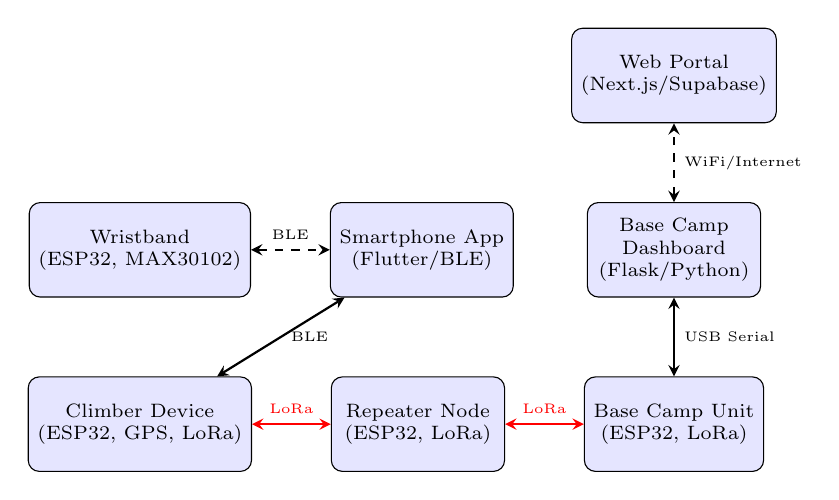
\begin{tikzpicture}[
        node distance=1cm and 1cm,
        box/.style={draw, rectangle, rounded corners, minimum width=2.2cm, minimum height=1.2cm, align=center, fill=blue!10, font=\scriptsize},
        arrow/.style={thick, ->, >=stealth}
    ]
        % Nodes
        \node[box] (wristband) {Wristband\\(ESP32, MAX30102)};
        \node[box, right=of wristband] (phone) {Smartphone App\\(Flutter/BLE)};
        \node[box, below=of wristband] (climber) {Climber Device\\(ESP32, GPS, LoRa)};
        \node[box, right=of climber] (repeater) {Repeater Node\\(ESP32, LoRa)};
        \node[box, right=of repeater] (basecamp) {Base Camp Unit\\(ESP32, LoRa)};
        \node[box, above=of basecamp] (dashboard) {Base Camp\\Dashboard\\(Flask/Python)};
        \node[box, above=of dashboard] (portal) {Web Portal\\(Next.js/Supabase)};

        % Connections
        \draw[arrow, <->, dashed] (wristband) -- node[above, font=\tiny] {BLE} (phone);
        \draw[arrow, <->] (phone) -- node[right, font=\tiny] {BLE} (climber);
        \draw[arrow, <->, thick, red] (climber) -- node[above, font=\tiny] {LoRa} (repeater);
        \draw[arrow, <->, thick, red] (repeater) -- node[above, font=\tiny] {LoRa} (basecamp);
        \draw[arrow, <->, thick] (basecamp) -- node[right, font=\tiny] {USB Serial} (dashboard);
        \draw[arrow, <->, dashed] (dashboard) -- node[right, font=\tiny] {WiFi/Internet} (portal);
        
    \end{tikzpicture}
    \caption{High-Level System Architecture and Interconnections}
    \label{fig:system-architecture}
\end{figure}

\begin{infobox}
The system operates completely independently of cellular networks during an expedition. Internet connectivity is only required for the Web Portal, which is used pre- and post-expedition for device registration and data sync.
\end{infobox}

\section{Data Flow Architecture}
Data flows through the system in two primary pipelines: health telemetry and geographical tracking/messaging.

\begin{figure}[htbp]
    \centering
    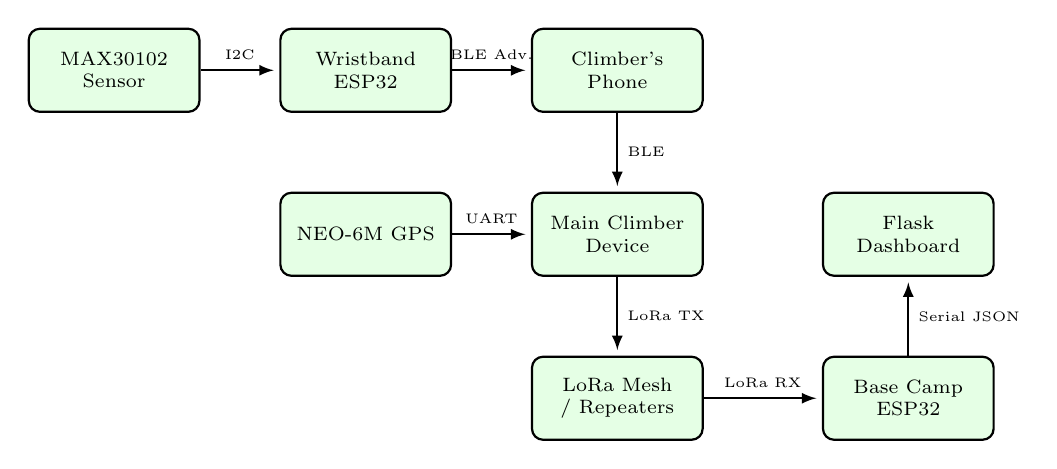
\begin{tikzpicture}[
        auto,
        block/.style={rectangle, draw=black, thick, fill=green!10, text width=5.5em, text centered, rounded corners, minimum height=3em, font=\scriptsize},
        line/.style={draw, thick, -latex, shorten >=2pt}
    ]
        % Define nodes
        \node [block] (sensor) {MAX30102 Sensor};
        \node [block, right=1cm of sensor] (wristband) {Wristband ESP32};
        \node [block, right=1cm of wristband] (phone) {Climber's Phone};
        \node [block, below=1cm of phone] (climber) {Main Climber Device};
        \node [block, left=1cm of climber] (gps) {NEO-6M GPS};
        \node [block, below=1cm of climber] (lora_mesh) {LoRa Mesh / Repeaters};
        \node [block, right=1.5cm of lora_mesh] (base_esp) {Base Camp ESP32};
        \node [block, above=1cm of base_esp] (dashboard) {Flask Dashboard};

        % Draw edges
        \path [line] (sensor) -- node[above, font=\tiny] {I2C} (wristband);
        \path [line] (wristband) -- node[above, font=\tiny] {BLE Adv.} (phone);
        \path [line] (phone) -- node[right, font=\tiny] {BLE} (climber);
        \path [line] (gps) -- node[above, font=\tiny] {UART} (climber);
        \path [line] (climber) -- node[right, font=\tiny] {LoRa TX} (lora_mesh);
        \path [line] (lora_mesh) -- node[above, font=\tiny] {LoRa RX} (base_esp);
        \path [line] (base_esp) -- node[right, font=\tiny] {Serial JSON} (dashboard);
        
    \end{tikzpicture}
    \caption{Detailed Data Flow Diagram}
    \label{fig:data-flow}
\end{figure}

The data flow begins at the edges:
\begin{enumerate}
    \item \textbf{Health Data:} The MAX30102 sensor on the Wristband reads raw photoplethysmogram (PPG) data, which the ESP32 processes to calculate Heart Rate and SpO$_2$. This data is advertised via BLE.
    \item \textbf{Local Aggregation:} The climber's mobile phone app scans for these BLE advertisements, displaying the vitals locally.
    \item \textbf{Transmission Prep:} The Main Climber Device, which is paired via BLE to the phone and directly reading GPS data via UART, constructs data packets containing the GPS coordinates, health vitals (received via the phone or direct BLE), and system status.
    \item \textbf{Long-Range Transmission:} These packets are broadcast over the 433 MHz LoRa interface.
    \item \textbf{Relay:} Repeater nodes pick up the LoRa packets and re-broadcast them, extending the range over rough terrain.
    \item \textbf{Reception \& Display:} The Base Camp Unit receives the LoRa packets, formats them into a serialized JSON structure, and pushes them over a USB serial connection (at 115200 baud) to the laptop running the Python Flask dashboard, which renders the data on an HTML5 canvas map.
\end{enumerate}

\section{Deployment Strategy in Mountainous Terrain}
The physical deployment of the hardware is critical to the system's success. LoRa, operating at 433 MHz, requires line-of-sight (LoS) or near-LoS for maximum range. In a mountain setting, valleys and ridges obstruct radio waves. 

\begin{figure}[htbp]
    \centering
    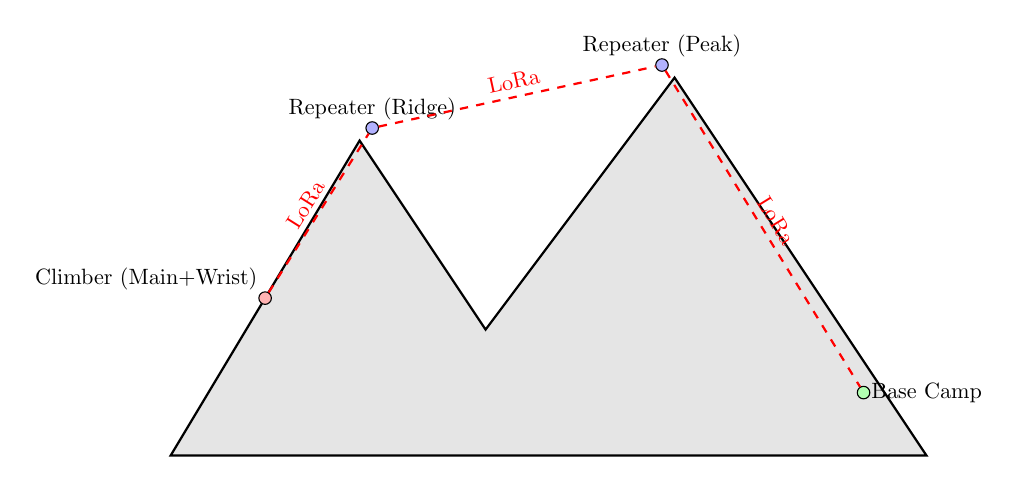
\begin{tikzpicture}[scale=0.8, transform shape]
        % Mountain drawing
        \draw[thick, fill=gray!20] (0,0) -- (3,5) -- (5,2) -- (8,6) -- (12,0) -- cycle;
        
        % Nodes
        \node[circle, draw, fill=red!30, inner sep=2pt] (climber) at (1.5,2.5) {};
        \node[above left] at (climber) {Climber (Main+Wrist)};
        
        \node[circle, draw, fill=blue!30, inner sep=2pt] (repeater1) at (3.2,5.2) {};
        \node[above] at (repeater1) {Repeater (Ridge)};
        
        \node[circle, draw, fill=blue!30, inner sep=2pt] (repeater2) at (7.8,6.2) {};
        \node[above] at (repeater2) {Repeater (Peak)};
        
        \node[circle, draw, fill=green!30, inner sep=2pt] (base) at (11,1) {};
        \node[right] at (base) {Base Camp};
        
        % LoRa links
        \draw[dashed, thick, red] (climber) -- node[above, sloped] {LoRa} (repeater1);
        \draw[dashed, thick, red] (repeater1) -- node[above, sloped] {LoRa} (repeater2);
        \draw[dashed, thick, red] (repeater2) -- node[above, sloped] {LoRa} (base);
        
    \end{tikzpicture}
    \caption{Deployment diagram illustrating the role of Repeaters in overcoming mountain topology}
    \label{fig:deployment}
\end{figure}

To overcome this, \textbf{Repeater Nodes} are strategically placed at high elevation points (e.g., ridges or peaks) during the ascent. These nodes act as relay stations. The base camp is typically located in a valley, and the climber may be on the other side of a ridge. The repeater on the ridge ensures continuous communication by acting as a bridge between the climber and the base camp.

\chapter{Hardware Design}
\label{ch:hardware-design}

This chapter details the hardware architecture, component selection, circuit design, and power management strategies for the four distinct physical devices comprising the system.

\section{Component Specifications}
Across the devices, standard modules were chosen for reliability, availability, and community support:
\begin{itemize}
    \item \textbf{ESP32 Microcontroller:} The core processing unit. Features a dual-core Tensilica LX6 microprocessor running at 240 MHz, 520 KB internal SRAM, and integrated Wi-Fi (802.11 b/g/n) and Bluetooth (v4.2 BR/EDR and BLE). Operating voltage is 3.3V.
    \item \textbf{MAX30102 Sensor:} An integrated pulse oximetry and heart-rate monitor module. It communicates via I2C and operates strictly at 3.3V.
    \item \textbf{NEO-6M GPS Module:} A cost-effective, high-performance GPS receiver with a built-in ceramic antenna. It communicates via UART (default 9600 baud rate).
    \item \textbf{SX1278 LoRa Transceiver:} A long-range wireless transceiver operating at the 433 MHz ISM band. It interfaces with the ESP32 via SPI and is crucial for the mesh network.
\end{itemize}

\section{Climber Main Device}
The Climber Main Device acts as the central hub for the user, aggregating local data and handling long-range communications.

\subsection{Design Rationale}
This device requires significant processing capability to manage BLE connections with the phone, UART communication with the GPS, and SPI communication with the LoRa module simultaneously. The ESP32 is perfectly suited for this due to its dual-core nature and RTOS support. 

\subsection{Electronic Schematic \& PCB Layout}

\begin{figure}[htbp]
    \centering
    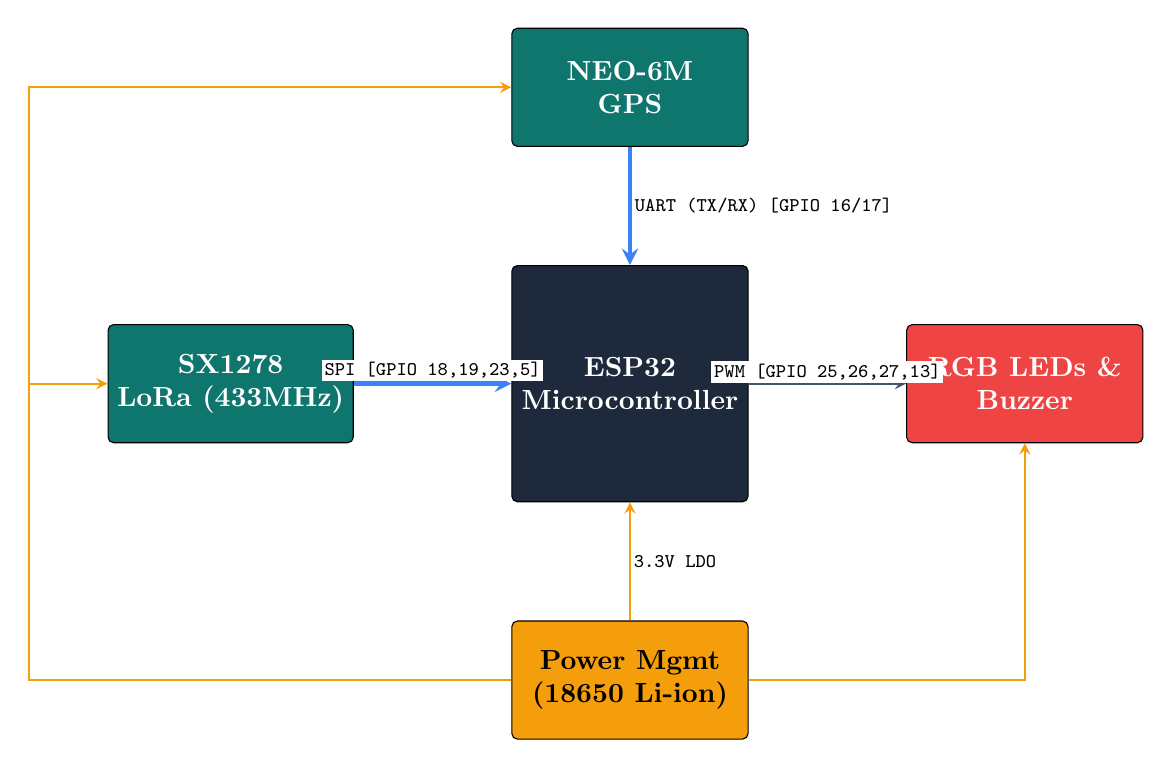
\begin{tikzpicture}[
        node distance=1.5cm and 1.5cm,
        chip/.style={draw, rectangle, rounded corners=2pt, minimum width=3cm, minimum height=1.5cm, align=center, fill=slate800, text=white, font=\bfseries},
        wire/.style={-stealth, thick, draw=slate600},
        bus/.style={-stealth, ultra thick, draw=blue500},
        label/.style={font=\scriptsize\ttfamily, fill=white, inner sep=1pt}
    ]
        % Main MCU
        \node[chip, minimum height=3cm] (esp) {ESP32\\Microcontroller};
        
        % Peripherals
        \node[chip, fill=teal700, above=1.5cm of esp] (gps) {NEO-6M\\GPS};
        \node[chip, fill=teal700, left=2cm of esp] (lora) {SX1278\\LoRa (433MHz)};
        \node[chip, fill=red500, right=2cm of esp] (leds) {RGB LEDs \&\\Buzzer};
        \node[chip, fill=amber500, text=black, below=1.5cm of esp] (power) {Power Mgmt\\(18650 Li-ion)};

        % Signal Buses
        \draw[bus] (gps.south) -- node[label, right] {UART (TX/RX) [GPIO 16/17]} (esp.north);
        \draw[bus] (lora.east) -- node[label, above] {SPI [GPIO 18,19,23,5]} (esp.west);
        \draw[wire] (esp.east) -- node[label, above] {PWM [GPIO 25,26,27,13]} (leds.west);
        
        % Power Lines
        \draw[wire, draw=amber500, thick] (power.north) -- node[label, right] {3.3V LDO} (esp.south);
        \draw[wire, draw=amber500, thick] (power.east) -| (leds.south);
        
        % Power rail around the left
        \draw[wire, draw=amber500, thick] (power.west) -| ([xshift=-1cm]lora.west) |- (gps.west);
        \draw[wire, draw=amber500, thick] ([xshift=-1cm]lora.west |- lora.west) -- (lora.west);
    \end{tikzpicture}
    \caption{Climber Main Device Electronic Schematic}
    \label{fig:climber-schematic}
\end{figure}

\subsection{Power Supply \& PCB Considerations}
Powered by a single 18650 Lithium-ion battery (3.7V nominal, 3400mAh). A low-dropout (LDO) linear regulator (AMS1117-3.3) steps the battery voltage down to the 3.3V required by the ESP32 and peripherals. 

\textbf{PCB Trace Routing:}
\begin{itemize}
    \item \textbf{SPI Integrity:} The traces for the SX1278 SPI bus (SCK, MISO, MOSI) are kept under 30mm to prevent signal degradation and crosstalk. Right-angle bends are avoided to maintain impedance continuity.
    \item \textbf{RF Antenna Path:} The trace connecting the SX1278 ANT pin to the SMA connector is designed as a 50$\Omega$ coplanar waveguide with ground shielding.
    \item \textbf{Thermal Dissipation:} Large copper pours are utilized around the AMS1117 regulator to act as a heat sink.
\end{itemize}

\section{Wristband Device}
\subsection{Design Rationale}
The wristband requires a compact form factor. It dedicatedly reads health vitals and advertises them over BLE, allowing it to use a smaller battery footprint.

\subsection{Electronic Schematic}

\begin{figure}[htbp]
    \centering
    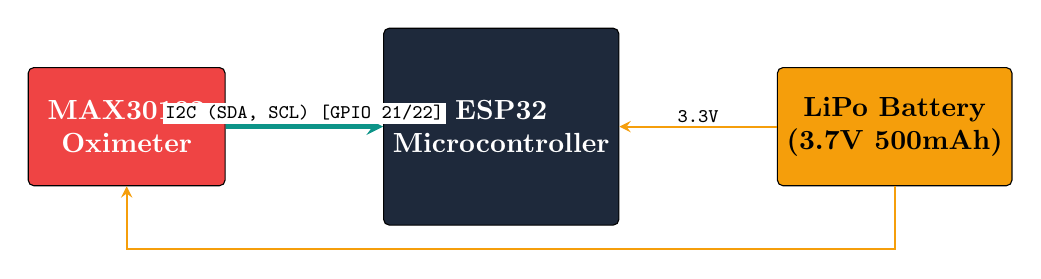
\begin{tikzpicture}[
        node distance=1.5cm and 2cm,
        chip/.style={draw, rectangle, rounded corners=2pt, minimum width=2.5cm, minimum height=1.5cm, align=center, fill=slate800, text=white, font=\bfseries},
        wire/.style={-stealth, thick, draw=slate600},
        bus/.style={-stealth, ultra thick, draw=teal600},
        label/.style={font=\scriptsize\ttfamily, fill=white, inner sep=1pt}
    ]
        % Main MCU
        \node[chip, minimum height=2.5cm] (esp) {ESP32\\Microcontroller};
        
        % Peripherals
        \node[chip, fill=red500, left=of esp] (sensor) {MAX30102\\Oximeter};
        \node[chip, fill=amber500, text=black, right=of esp] (power) {LiPo Battery\\(3.7V 500mAh)};

        % I2C Bus
        \draw[bus] (sensor.east) -- node[label, above] {I2C (SDA, SCL) [GPIO 21/22]} (esp.west);
        
        % Power Lines
        \draw[wire, draw=amber500, thick] (power.west) -- node[label, above] {3.3V} (esp.east);
        
        % Sensor power
        \draw[wire, draw=amber500, thick] (power.south) -- +(0,-0.8) -| (sensor.south);
    \end{tikzpicture}
    \caption{Wristband Device Electronic Schematic}
    \label{fig:wristband-schematic}
\end{figure}

\section{Repeater Node}
\subsection{Design Rationale}
The Repeater node is essentially a stripped-down version of the main device, consisting only of the ESP32, SX1278 LoRa module, and a larger battery capacity (dual 18650s in parallel) since it must remain active for the duration of the expedition on a remote ridge.

\subsection{Electronic Schematic}

\begin{figure}[htbp]
    \centering
    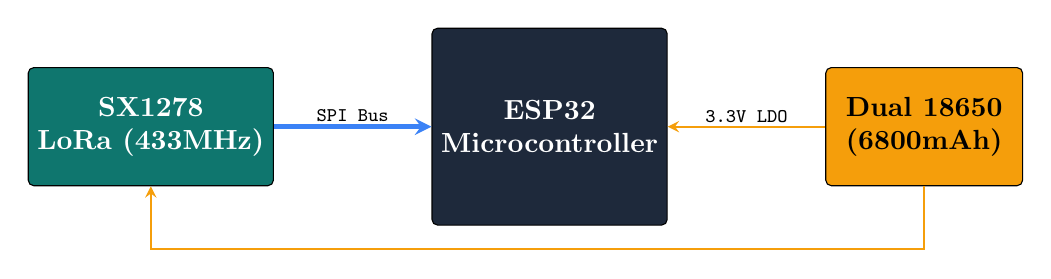
\begin{tikzpicture}[
        node distance=1.5cm and 2cm,
        chip/.style={draw, rectangle, rounded corners=2pt, minimum width=2.5cm, minimum height=1.5cm, align=center, fill=slate800, text=white, font=\bfseries},
        wire/.style={-stealth, thick, draw=slate600},
        bus/.style={-stealth, ultra thick, draw=blue500},
        label/.style={font=\scriptsize\ttfamily, fill=white, inner sep=1pt}
    ]
        % Main MCU
        \node[chip, minimum height=2.5cm] (esp) {ESP32\\Microcontroller};
        
        % Peripherals
        \node[chip, fill=teal700, left=of esp] (lora) {SX1278\\LoRa (433MHz)};
        \node[chip, fill=amber500, text=black, right=of esp] (power) {Dual 18650\\(6800mAh)};

        % SPI Bus
        \draw[bus] (lora.east) -- node[label, above] {SPI Bus} (esp.west);
        
        % Power Lines
        \draw[wire, draw=amber500, thick] (power.west) -- node[label, above] {3.3V LDO} (esp.east);
        \draw[wire, draw=amber500, thick] (power.south) -- +(0,-0.8) -| (lora.south);
        
    \end{tikzpicture}
    \caption{Repeater Node Electronic Schematic}
    \label{fig:repeater-schematic}
\end{figure}

\section{Base Camp Unit}
\subsection{Design Rationale}
The Base Camp Unit mirrors the Repeater hardware but operates in a different software mode. It requires a stable serial data connection to the laptop running the Dashboard.

\subsection{Electronic Schematic}

\begin{figure}[htbp]
    \centering
    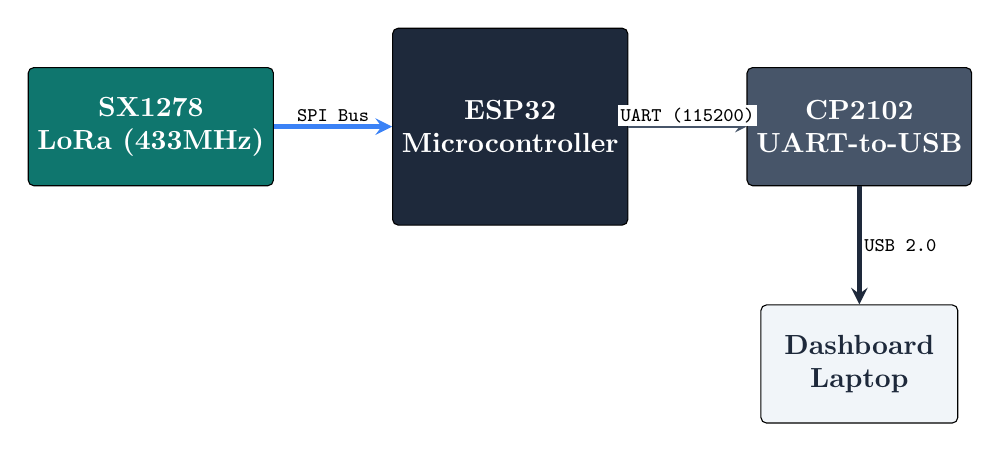
\begin{tikzpicture}[
        node distance=1.5cm and 1.5cm,
        chip/.style={draw, rectangle, rounded corners=2pt, minimum width=2.5cm, minimum height=1.5cm, align=center, fill=slate800, text=white, font=\bfseries},
        wire/.style={-stealth, thick, draw=slate600},
        bus/.style={-stealth, ultra thick, draw=blue500},
        label/.style={font=\scriptsize\ttfamily, fill=white, inner sep=1pt}
    ]
        % Main MCU
        \node[chip, minimum height=2.5cm] (esp) {ESP32\\Microcontroller};
        
        % Peripherals
        \node[chip, fill=teal700, left=of esp] (lora) {SX1278\\LoRa (433MHz)};
        \node[chip, fill=slate600, right=of esp] (usb) {CP2102\\UART-to-USB};
        \node[chip, fill=chaptergray, text=slate800, below=of usb] (laptop) {Dashboard\\Laptop};

        % SPI Bus
        \draw[bus] (lora.east) -- node[label, above] {SPI Bus} (esp.west);
        
        % Serial Bus
        \draw[wire, thick] (esp.east) -- node[label, above] {UART (115200)} (usb.west);
        \draw[bus, draw=slate800] (usb.south) -- node[label, right] {USB 2.0} (laptop.north);
        
    \end{tikzpicture}
    \caption{Base Camp Unit Electronic Schematic}
    \label{fig:basecamp-schematic}
\end{figure}

\begin{cautionbox}
Ensure that the Base Camp Unit's LoRa antenna is properly connected before powering on via USB. Transmitting LoRa signals without an antenna connected can irreversibly damage the SX1278 transceiver amplifier due to impedance mismatch.
\end{cautionbox}

\chapter{Communication Protocol Design}
\label{ch:communication-protocols}

This chapter outlines the proprietary data formats, transmission settings, and protocols developed to ensure reliable data flow across the heterogeneous network interfaces used in the system.

\section{LoRa Mesh Protocol}
The backbone of the system's off-grid communication is the 433 MHz LoRa network. Rather than a simple point-to-point link, the system implements a rudimentary mesh/relay logic to overcome the topological challenges of mountainous environments.

\subsection{LoRa Radio Settings}
\begin{itemize}
    \item \textbf{Frequency:} 433 MHz (ISM band suitable for high obstacle penetration).
    \item \textbf{Spreading Factor (SF):} SF7. This was chosen as a compromise. While SF12 offers the maximum range, it drastically increases the Time on Air (ToA), leading to packet collisions in a mesh setup. SF7 provides sufficient range when combined with repeaters while keeping transmission times short.
    \item \textbf{Bandwidth (BW):} 125 kHz. Standard bandwidth balancing range and data rate.
    \item \textbf{Coding Rate (CR):} 4/5. Provides minimal forward error correction, reducing overhead since the mesh logic implements its own packet acknowledgment and retry mechanisms.
\end{itemize}

\subsection{Packet Format}
All LoRa transmissions adhere to a custom binary packet structure to minimize payload size. 

\begin{figure}[htbp]
    \centering
    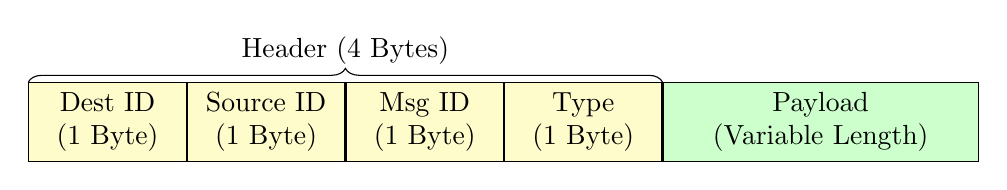
\begin{tikzpicture}[
        cell/.style={draw, rectangle, minimum height=1cm, align=center, fill=yellow!20},
        node distance=0cm
    ]
        \node[cell, minimum width=2cm] (dest) {Dest ID\\(1 Byte)};
        \node[cell, minimum width=2cm, right=of dest] (src) {Source ID\\(1 Byte)};
        \node[cell, minimum width=2cm, right=of src] (msgId) {Msg ID\\(1 Byte)};
        \node[cell, minimum width=2cm, right=of msgId] (type) {Type\\(1 Byte)};
        \node[cell, minimum width=4cm, right=of type, fill=green!20] (payload) {Payload\\(Variable Length)};
        
        \draw [decorate,decoration={brace,amplitude=5pt},xshift=0pt,yshift=2pt]
        (dest.north west) -- (type.north east) node [black,midway,yshift=0.4cm] {Header (4 Bytes)};
    \end{tikzpicture}
    \caption{LoRa Packet Structure}
    \label{fig:lora-packet}
\end{figure}

\subsection{Message Types}
The \texttt{Type} byte dictates how the payload is parsed:
\begin{itemize}
    \item \texttt{0x01 (SOS):} Highest priority. Payload contains critical GPS and vital data. Nodes relay this immediately.
    \item \texttt{0x02 (GPS):} Standard location update.
    \item \texttt{0x03 (HEARTBEAT):} Sent periodically to update node routing tables and signify device online status.
    \item \texttt{0x04 (TEXT):} Custom string messages sent from the mobile app to the dashboard, or vice-versa.
\end{itemize}

\subsection{Relay and Routing Logic}
When a node receives a packet:
\begin{enumerate}
    \item It checks if the \texttt{Dest ID} matches its own ID. If yes, it processes the packet.
    \item If not, it checks a local buffer to see if it has recently forwarded this \texttt{Msg ID} from this \texttt{Source ID}.
    \item If not forwarded recently, it rebroadcasts the packet, decrementing a Time-To-Live (TTL) counter (embedded in the payload for standard messages) to prevent infinite loops.
\end{enumerate}

\section{BLE Protocol}
The Wristband communicates with the Climber's phone via Bluetooth Low Energy (BLE). 
The ESP32 on the wristband acts as a BLE Peripheral, hosting a custom GATT (Generic Attribute Profile) Server.
\begin{itemize}
    \item \textbf{Service UUID:} \texttt{4fafc201-1fb5-459e-8fcc-c5c9c331914b}
    \item \textbf{Heart Rate Characteristic:} \texttt{beb5483e-36e1-4688-b7f5-ea07361b26a8} (Notify, Read)
    \item \textbf{SpO2 Characteristic:} \texttt{8a7c2936-e8cc-4d37-84be-5bdba349e59d} (Notify, Read)
\end{itemize}
The sensor data is packed into byte arrays and pushed to the phone via GATT notifications at a frequency of 1 Hz.

\section{WiFi and HTTP Protocol}
The Base Camp Unit operates in WiFi SoftAP (Software Access Point) mode if a wireless connection to the dashboard is preferred over USB serial. It hosts a lightweight asynchronous web server.
\begin{lstlisting}[language=C++, caption={ESP32 SoftAP Configuration Snippet}]
WiFi.softAP("BaseCamp_Network", "mountain123");
IPAddress IP = WiFi.softAPIP();
\end{lstlisting}
The HTTP server exposes RESTful endpoints:
\begin{itemize}
    \item \texttt{GET /data} - Returns the latest JSON array of received LoRa packets.
    \item \texttt{POST /send} - Accepts JSON payloads from the dashboard to be broadcasted via LoRa to climbers.
\end{itemize}

\section{Serial JSON Protocol}
The primary and most robust link between the Base Camp ESP32 and the Python Flask Dashboard is a direct USB Serial connection operating at \texttt{115200} baud. Data received from the LoRa mesh is encapsulated into JSON objects and printed to the serial port.

\begin{lstlisting}[caption={Example Serial JSON Packet}]
{
  "timestamp": 1694770000,
  "source_id": "CLIMBER_01",
  "type": "GPS_VITALS",
  "data": {
    "lat": 7.2906,
    "lng": 80.6337,
    "hr": 85,
    "spo2": 96
  },
  "rssi": -92
}
\end{lstlisting}
The Flask application runs a background thread that continuously reads the serial port, parses these JSON packets, and emits them to the web frontend using WebSockets.

\chapter{Firmware Design}
\label{ch:firmware_design}

This chapter details the firmware design for the microcontrollers operating within the Mountain Climber Health \& GPS Tracker system. The firmware handles critical tasks including sensor data acquisition, wireless communication (BLE and LoRa), power management, and real-time processing.

\section{Operational States}

The firmware on the Main Climber Device and the Wristband operates using finite state machines to ensure deterministic behavior and efficient power utilization.

\subsection{Main Climber Device State Machine}

The Main Climber Device acts as the central hub for a climber, coordinating between the wristband (via BLE) and the mesh network (via LoRa).

\begin{figure}[htbp]
    \centering
    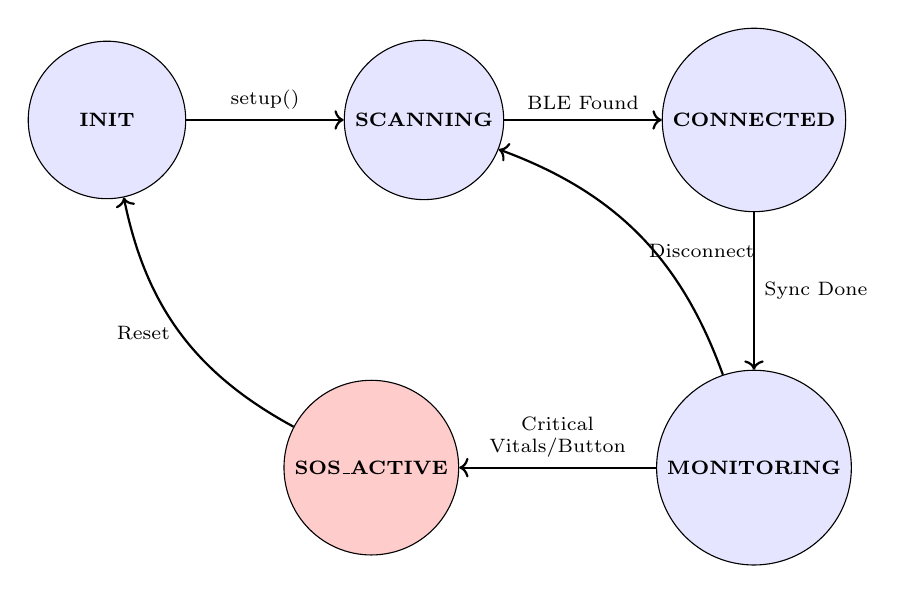
\begin{tikzpicture}[
        node distance = 1.5cm and 2cm,
        state/.style = {circle, draw, minimum size=2cm, align=center, fill=blue!10, font=\scriptsize\bfseries},
        edge/.style = {->, thick},
        label/.style = {font=\scriptsize, align=center}
    ]
    \node[state] (init) {INIT};
    \node[state, right=2cm of init] (scan) {SCANNING};
    \node[state, right=2cm of scan] (conn) {CONNECTED};
    \node[state, below=2cm of conn] (mon) {MONITORING};
    \node[state, left=2.5cm of mon, fill=red!20] (sos) {SOS\_ACTIVE};
    
    \draw[edge] (init) -- node[label, above] {setup()} (scan);
    \draw[edge] (scan) -- node[label, above] {BLE Found} (conn);
    \draw[edge] (conn) -- node[label, right] {Sync Done} (mon);
    \draw[edge, bend right=25] (mon) to node[label, below right] {Disconnect} (scan);
    \draw[edge] (mon) -- node[label, above] {Critical\\Vitals/Button} (sos);
    \draw[edge, bend left=25] (sos) to node[label, left] {Reset} (init);
    \end{tikzpicture}
    \caption{State Machine Diagram for Main Climber Device}
    \label{fig:main_state_machine}
\end{figure}

\subsection{Wristband State Machine}

The wristband's primary role is to acquire health data and transmit it via BLE.

\begin{figure}[htbp]
    \centering
    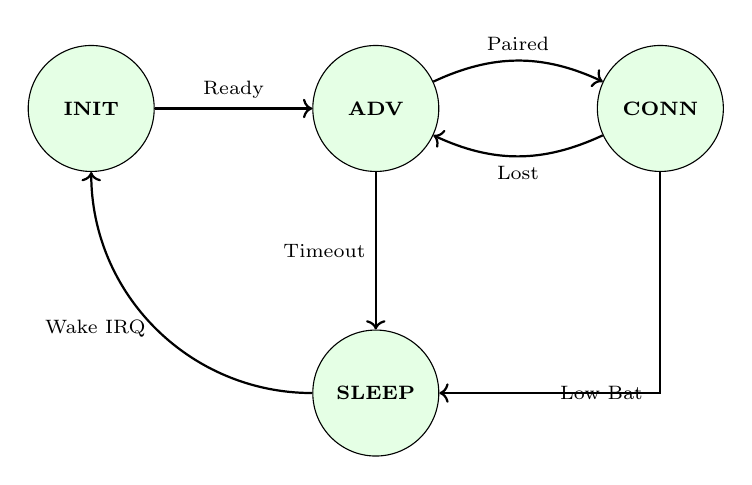
\begin{tikzpicture}[
        node distance = 2.5cm,
        state/.style = {circle, draw, minimum size=1.6cm, align=center, fill=green!10, font=\scriptsize\bfseries},
        edge/.style = {->, thick},
        label/.style = {font=\scriptsize, align=center}
    ]
    \node[state] (init) {INIT};
    \node[state, right=2cm of init] (adv) {ADV};
    \node[state, right=2cm of adv] (conn) {CONN};
    \node[state, below=2cm of adv] (sleep) {SLEEP};
    
    \draw[edge] (init) -- node[label, above] {Ready} (adv);
    \draw[edge, bend left=25] (adv) to node[label, above] {Paired} (conn);
    \draw[edge, bend left=25] (conn) to node[label, below] {Lost} (adv);
    \draw[edge] (adv) -- node[label, left] {Timeout} (sleep);
    \draw[edge] (conn) |- node[label, near end, right] {Low Bat} (sleep);
    \draw[edge, bend left=45] (sleep) to node[label, left] {Wake IRQ} (init);
    \end{tikzpicture}
    \caption{State Machine Diagram for Wristband}
    \label{fig:wristband_state_machine}
\end{figure}

\section{Key Algorithms}

\subsection{Distance Calculation (Haversine Formula)}

To calculate the distance between climbers or between a climber and the base camp, the firmware utilizes the Haversine formula. This computes the great-circle distance between two points on a sphere given their longitudes and latitudes.

The formula is defined as:
\begin{equation}
a = \sin^2\left(\frac{\Delta \varphi}{2}\right) + \cos \varphi_1 \cdot \cos \varphi_2 \cdot \sin^2\left(\frac{\Delta \lambda}{2}\right)
\end{equation}
\begin{equation}
c = 2 \cdot \text{atan2}\left(\sqrt{a}, \sqrt{1-a}\right)
\end{equation}
\begin{equation}
d = R \cdot c
\end{equation}
Where:
\begin{itemize}
    \item $\varphi_1, \varphi_2$ are the latitudes of point 1 and point 2 (in radians).
    \item $\Delta \varphi = \varphi_2 - \varphi_1$
    \item $\Delta \lambda = \lambda_2 - \lambda_1$ (difference in longitude, in radians).
    \item $R$ is the Earth's radius (mean radius = 6,371 km).
\end{itemize}

\subsection{Health Threshold Detection}

The firmware continuously evaluates the readings from the MAX30102 sensor. Normal heart rates typically fall between 60 to 100 bpm, while SpO2 levels should ideally remain above 95\%. In high-altitude environments, SpO2 can naturally drop, but dangerous hypoxia must be identified.

The threshold algorithm triggers an automatic SOS alert if:
\begin{itemize}
    \item Heart Rate (HR) $< 40$ bpm OR HR $> 120$ bpm
    \item SpO2 $< 90\%$
\end{itemize}

\begin{lstlisting}[language=C++, caption={Health Threshold Checking Algorithm}, label={lst:health_check}]
void checkHealthThresholds(int hr, int spo2) {
    bool isEmergency = false;
    
    if (hr < 40 || hr > 120) {
        isEmergency = true;
        logWarning("Abnormal Heart Rate detected!");
    }
    
    if (spo2 < 90 && spo2 > 0) { // Ignore 0 which means no finger attached
        isEmergency = true;
        logWarning("Low SpO2 detected!");
    }
    
    if (isEmergency) {
        triggerAutomaticSOS();
    }
}
\end{lstlisting}

\subsection{NMEA GPS Sentence Parsing}

The NEO-6M GPS module outputs data in NMEA 0183 format. The firmware primarily parses the \$GPRMC (Recommended Minimum Specific GPS/TRANSIT Data) and \$GPGGA (Global Positioning System Fix Data) sentences to extract latitude, longitude, and altitude.

\subsection{LoRa Packet Assembly and Disassembly}

Data transmitted over the 433MHz LoRa network is structured to minimize payload size while ensuring reliable delivery. 

\begin{infobox}
The LoRa settings used are: Spreading Factor (SF) 7, Bandwidth (BW) 125kHz, and Coding Rate (CR) 4/5. These settings provide a balanced trade-off between range and data rate.
\end{infobox}

A typical packet structure includes:
\begin{itemize}
    \item \textbf{Header}: Node ID, Packet Type (SOS, GPS, VITALS, TEXT).
    \item \textbf{Payload}: Formatted data bytes.
    \item \textbf{Checksum}: Simple CRC for integrity verification.
\end{itemize}

\section{System Configurations}

\subsection{Interrupt Handling Strategy}
Hardware interrupts are utilized for time-critical events to prevent polling overhead. 
\begin{itemize}
    \item \textbf{MAX30102 Data Ready}: Triggers an interrupt when a new sample is available, waking the I2C read task.
    \item \textbf{LoRa DIO0}: Triggers on TxDone or RxDone, signaling the communication task.
    \item \textbf{SOS Button}: Configured as a high-priority falling-edge interrupt with hardware debouncing.
\end{itemize}

\subsection{Watchdog Timer Configuration}
To ensure system reliability, the ESP32 Hardware Watchdog Timer (WDT) is configured with a 5-second timeout. Core tasks (sensor reading, communications) must periodically reset the WDT. If a task hangs due to an I2C lockup or an infinite loop, the WDT resets the microcontroller, ensuring the device recovers in remote environments.

\subsection{Power Management}
Power management is critical for the 18650 Li-ion battery. The firmware employs ESP32's sleep modes:
\begin{itemize}
    \item \textbf{Light Sleep}: Used during idle periods where memory and state are preserved, but CPU clock is gated.
    \item \textbf{Deep Sleep}: Used in the wristband when detached. The device wakes up only via an external interrupt (wake-on-interrupt) triggered by the onboard accelerometer or a physical button press.
\end{itemize}

\chapter{Mobile Application Design}
\label{ch:mobile_app_design}

This chapter details the design of the mobile application developed for the Mountain Climber Health \& GPS Tracker system. Built using Flutter and Dart, the application provides climbers with real-time access to their health metrics, location data, and communication tools.

\section{Architecture}

The application follows a reactive architecture utilizing the standard Flutter widget tree paradigm combined with a robust state management solution.

\subsection{State Management}
The app employs the \textit{Provider} pattern for state management. This approach separates business logic from UI components, allowing different parts of the application to react to changes in BLE connection status, incoming sensor data, or new messages without requiring widespread widget rebuilds.

\section{BLE Scanning and Connection Flow}

The mobile application acts as a BLE Central device, scanning for and connecting to the Climber Main Device (acting as a BLE Peripheral).

\begin{figure}[H]
    \centering
    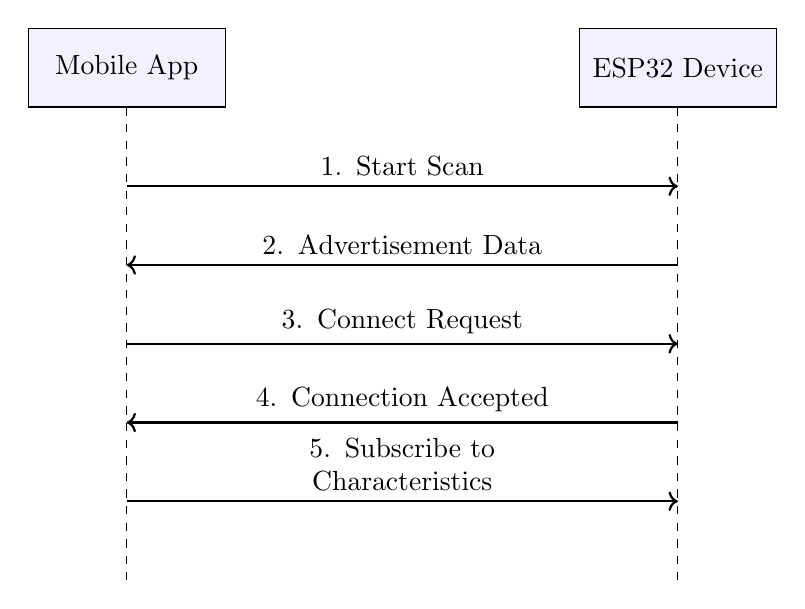
\begin{tikzpicture}[
        node distance=2cm,
        auto,
        box/.style={rectangle, draw, minimum width=2.5cm, minimum height=1cm, align=center, fill=blue!5},
        arrow/.style={->, thick}
    ]
    
    % Nodes
    \node[box] (app) {Mobile App};
    \node[box, right of=app, xshift=5cm] (device) {ESP32 Device};
    
    % Lifelines
    \draw[dashed] (app.south) -- +(0,-6cm);
    \draw[dashed] (device.south) -- +(0,-6cm);
    
    % Messages
    \draw[arrow] ([yshift=-1cm]app.south) -- node[above, text width=4cm, align=center] {1. Start Scan} ([yshift=-1cm]device.south);
    
    \draw[arrow] ([yshift=-2cm]device.south) -- node[above, text width=4cm, align=center] {2. Advertisement Data} ([yshift=-2cm]app.south);
    
    \draw[arrow] ([yshift=-3cm]app.south) -- node[above, text width=4cm, align=center] {3. Connect Request} ([yshift=-3cm]device.south);
    
    \draw[arrow] ([yshift=-4cm]device.south) -- node[above, text width=4cm, align=center] {4. Connection Accepted} ([yshift=-4cm]app.south);
    
    \draw[arrow] ([yshift=-5cm]app.south) -- node[above, text width=4cm, align=center] {5. Subscribe to Characteristics} ([yshift=-5cm]device.south);
    
    \end{tikzpicture}
    \caption{BLE Connection Sequence Diagram}
    \label{fig:ble_sequence}
\end{figure}

\subsection{Error Handling and Reconnection Strategy}
Mountainous environments are prone to interference that can drop BLE connections. The application implements an exponential backoff strategy for reconnection. If the connection drops, the app attempts to reconnect immediately. If that fails, it waits 2 seconds, then 4 seconds, up to a maximum interval, ensuring that battery life is not drained by continuous aggressive polling.

\section{Key Screens and UI Design Principles}

The UI is designed with high contrast and large touch targets, considering that climbers may be operating the app under harsh lighting conditions or while wearing gloves.

\subsection{Home Screen}
The Home screen serves as a dashboard summarizing the climber's status. It indicates the current BLE connection state and provides quick access to vital metrics and active alerts.

\begin{figure}[htbp]
    \centering
    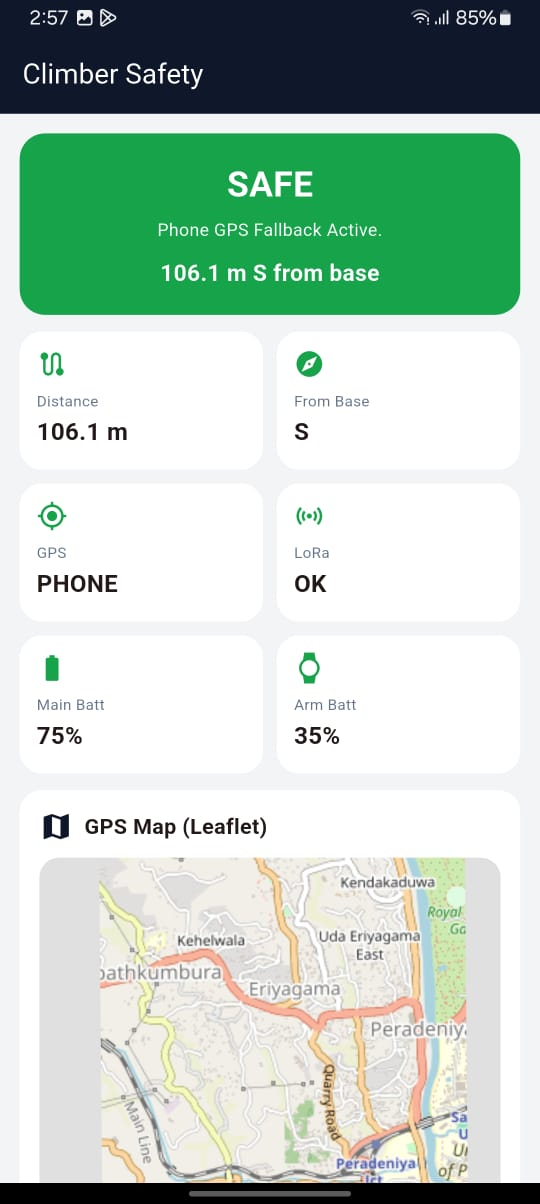
\includegraphics[width=0.8\textwidth]{app_home.png}
    \caption{Mobile App - Home Screen Interface}
    \label{fig:app_home}
\end{figure}

\subsection{Vitals Screen}
Displays real-time readings of Heart Rate, SpO2, and ambient temperature. Gauges and charts are used to show trends over time. Thresholds are color-coded (e.g., green for normal, red for critical).

\subsection{Map Screen}
Utilizes a custom painter in Flutter to render a specialized distance map. This map does not rely on internet map tiles (which are unavailable offline) but plots the relative positions of the user, the base camp, and other climbers based on received GPS coordinates and Haversine distance calculations.

\subsection{Messages Screen}
Provides a chat-like interface for two-way text messaging. Messages typed here are sent via BLE to the Climber Main Device, which relays them over the LoRa mesh network to the base camp or other climbers.

\section{Platform-Specific Configurations}

To utilize Bluetooth hardware, platform-specific permissions must be explicitly requested.

\subsection{Android Manifest}
The \texttt{AndroidManifest.xml} requires permissions for scanning, connecting, and accessing location (historically required for BLE scans on Android).
\begin{lstlisting}[language=XML, caption={Android BLE Permissions}, label={lst:android_permissions}]
<uses-permission android:name="android.permission.BLUETOOTH_SCAN" android:usesPermissionFlags="neverForLocation" />
<uses-permission android:name="android.permission.BLUETOOTH_CONNECT" />
<uses-permission android:name="android.permission.ACCESS_FINE_LOCATION" />
\end{lstlisting}

\subsection{iOS Info.plist}
The iOS \texttt{Info.plist} must include usage descriptions explaining to the user why Bluetooth is required.
\begin{lstlisting}[language=XML, caption={iOS Info.plist BLE Usage Description}, label={lst:ios_permissions}]
<key>NSBluetoothAlwaysUsageDescription</key>
<string>This app requires Bluetooth to connect to the climber health tracker.</string>
<key>NSBluetoothPeripheralUsageDescription</key>
<string>This app requires Bluetooth to communicate with the tracker.</string>
\end{lstlisting}

\chapter{Dashboard Design}
\label{ch:dashboard_design}

The Base Camp Dashboard is a critical component operated by the expedition monitoring team. It provides a comprehensive overview of all climbers in the network, visualizing their health data, GPS locations, and managing communications.

\section{Application Architecture}

The dashboard is built using Python with the Flask web framework. It operates as a local web server, rendering an interactive frontend while managing serial communications with the Base Camp LoRa Receiver in the backend.

\subsection{Threading Model}

To prevent the web server from blocking while waiting for serial data, the application employs a multi-threaded architecture.

\begin{figure}[htbp]
    \centering
    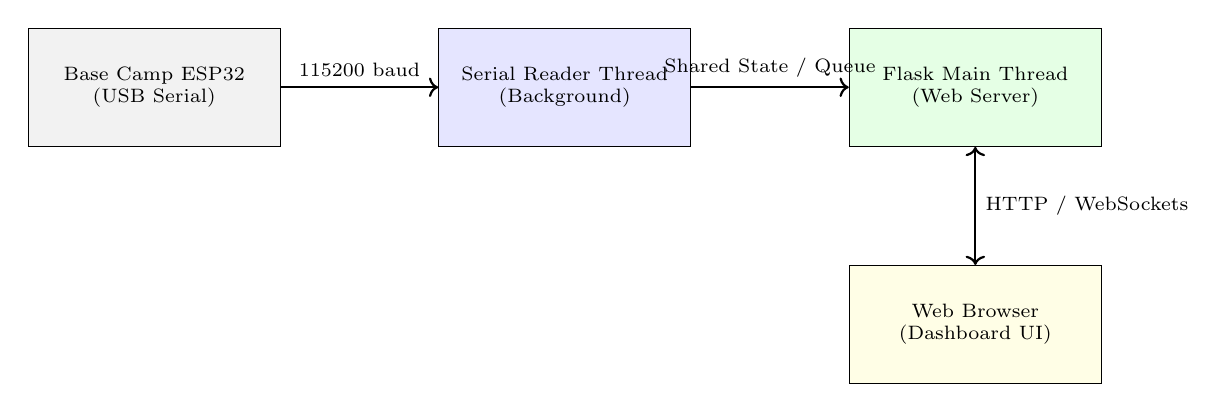
\begin{tikzpicture}[
        node distance=2.5cm,
        box/.style={rectangle, draw, minimum width=3.2cm, minimum height=1.5cm, align=center, fill=gray!10, font=\scriptsize},
        arrow/.style={->, thick},
        label/.style={font=\scriptsize, align=center}
    ]
    
    \node[box] (hardware) {Base Camp ESP32 \\ (USB Serial)};
    \node[box, right=2cm of hardware, fill=blue!10] (serial) {Serial Reader Thread \\ (Background)};
    \node[box, right=2cm of serial, fill=green!10] (flask) {Flask Main Thread \\ (Web Server)};
    \node[box, below=1.5cm of flask, fill=yellow!10] (client) {Web Browser \\ (Dashboard UI)};
    
    \draw[arrow] (hardware) -- node[label, above] {115200 baud} (serial);
    \draw[arrow] (serial) -- node[label, above] {Shared State / Queue} (flask);
    \draw[<->, thick] (flask) -- node[label, right] {HTTP / WebSockets} (client);
    
    \end{tikzpicture}
    \caption{Dashboard Threading Architecture}
    \label{fig:dashboard_threading}
\end{figure}

The \textbf{Serial Reader Thread} continuously reads JSON payloads from the USB serial port connected to the ESP32. It parses this data and updates a thread-safe shared state object. The \textbf{Flask Main Thread} handles incoming HTTP requests from the browser and serves the latest data from the shared state.

\section{Real-Time Map Rendering}

The dashboard features a live tracking map implemented using HTML5 Canvas.

\subsection{Coordinate Transformation}
Since the dashboard must operate completely offline without access to tile servers (like Google Maps or Mapbox), it plots climbers relative to the base camp. The Haversine formula is used to calculate the distance and bearing of each climber relative to the base camp's GPS origin. These polar coordinates are then converted to Cartesian coordinates $(x, y)$ and scaled to fit the HTML5 Canvas dimensions.

\subsection{Climber Marker Rendering}
The canvas dynamically renders markers for each climber. 
\begin{tipbox}
Markers are color-coded based on the climber's status: Green for normal, Orange for warning (e.g., missed heartbeat), and flashing Red for an active SOS.
\end{tipbox}

\section{SOS Alert Workflow}

Handling emergencies swiftly is the primary objective of the system.

\begin{figure}[htbp]
    \centering
    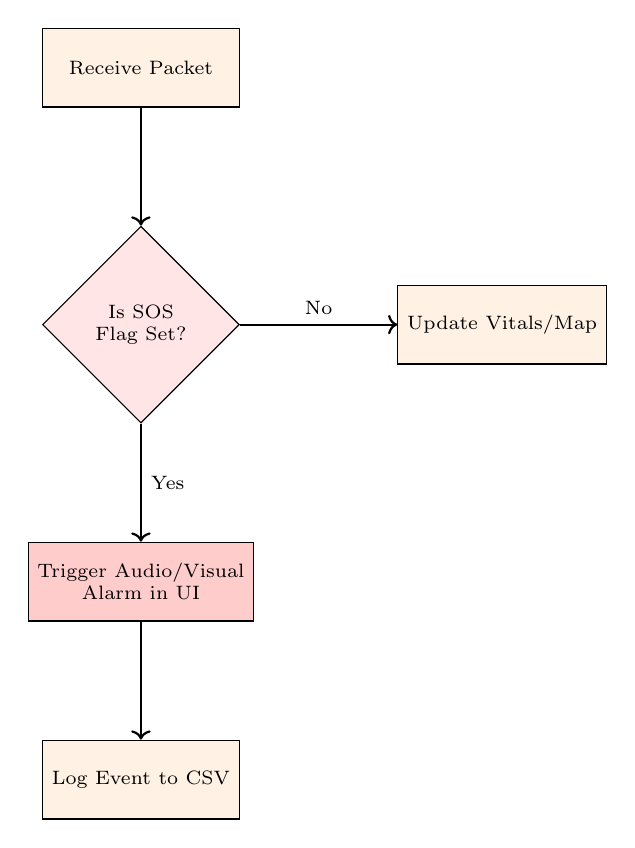
\begin{tikzpicture}[
        node distance=2cm,
        box/.style={rectangle, draw, minimum width=2.5cm, minimum height=1cm, align=center, fill=orange!10, font=\scriptsize},
        decision/.style={diamond, draw, minimum width=2.5cm, minimum height=2.5cm, align=center, fill=red!10, font=\scriptsize},
        arrow/.style={->, thick},
        label/.style={font=\scriptsize, align=center}
    ]
    
    \node[box] (receive) {Receive Packet};
    \node[decision, below=1.5cm of receive] (check) {Is SOS\\Flag Set?};
    \node[box, right=2cm of check] (normal) {Update Vitals/Map};
    \node[box, below=1.5cm of check, fill=red!20] (trigger) {Trigger Audio/Visual\\Alarm in UI};
    \node[box, below=1.5cm of trigger] (log) {Log Event to CSV};
    
    \draw[arrow] (receive) -- (check);
    \draw[arrow] (check) -- node[label, above] {No} (normal);
    \draw[arrow] (check) -- node[label, right] {Yes} (trigger);
    \draw[arrow] (trigger) -- (log);
    
    \end{tikzpicture}
    \caption{SOS Alert Processing Flowchart}
    \label{fig:sos_flowchart}
\end{figure}

\section{System Features}

\subsection{Two-Way Messaging}
The dashboard includes a chat interface. Messages typed in the web UI are sent via an API endpoint to the Flask backend, which formats them into a JSON payload and transmits them over the serial port to the Base Camp ESP32. The ESP32 then broadcasts the message over the LoRa network.

\subsection{CSV Export Logic}
For post-expedition analysis, all received data is logged. The backend utilizes Python's built-in \texttt{csv} module to append incoming sensor data, GPS coordinates, and timestamps to a daily log file, ensuring no data is lost during the mission.

\subsection{Packaging and Deployment}
The decision was made to embed the HTML, CSS, and JS directly within Python strings (or simple templates) rather than managing a separate frontend build process. This simplifies deployment. The entire Flask application, including the embedded web assets, is compiled into a single executable binary using \textbf{PyInstaller}. This allows expedition staff to run the dashboard on Windows or macOS laptops simply by double-clicking an executable, without needing to install Python or configure environments.

\chapter{Web Portal Design}
\label{ch:portal_design}

The web portal serves as the commercial and administrative front-end for the Mountain Climber Health \& GPS Tracker project, operating under the "Summit Gear" brand. It handles e-commerce for climbing equipment, device registration, and firmware distribution.

\section{Architecture}

The portal is built using \textbf{Next.js} utilizing the App Router architecture, backed by \textbf{Supabase} for database and authentication services.

\subsection{Server vs. Client Component Strategy}
Next.js 13+ introduced React Server Components. The portal leverages this by:
\begin{itemize}
    \item \textbf{Server Components (Default)}: Used for fetching product catalogs, rendering SEO-heavy pages, and handling database queries securely on the server. This reduces the JavaScript bundle size shipped to the client.
    \item \textbf{Client Components}: Explicitly marked with \texttt{"use client"}, these are used only where interactivity is required, such as the shopping cart, checkout forms, and real-time dashboard filtering.
\end{itemize}

\section{Supabase Integration}

Supabase provides a PostgreSQL database and an authentication layer.
\begin{itemize}
    \item \textbf{Server-Side Client}: Used in Next.js API routes and Server Components for secure data fetching (e.g., retrieving user orders) utilizing Server-Side Rendering (SSR).
    \item \textbf{Browser Client}: Used in Client Components for real-time updates (e.g., listening to stock changes) and handling client-side authentication states.
\end{itemize}

\section{Authentication Flow}

The portal utilizes Supabase Auth for managing users securely.

\begin{figure}[H]
    \centering
    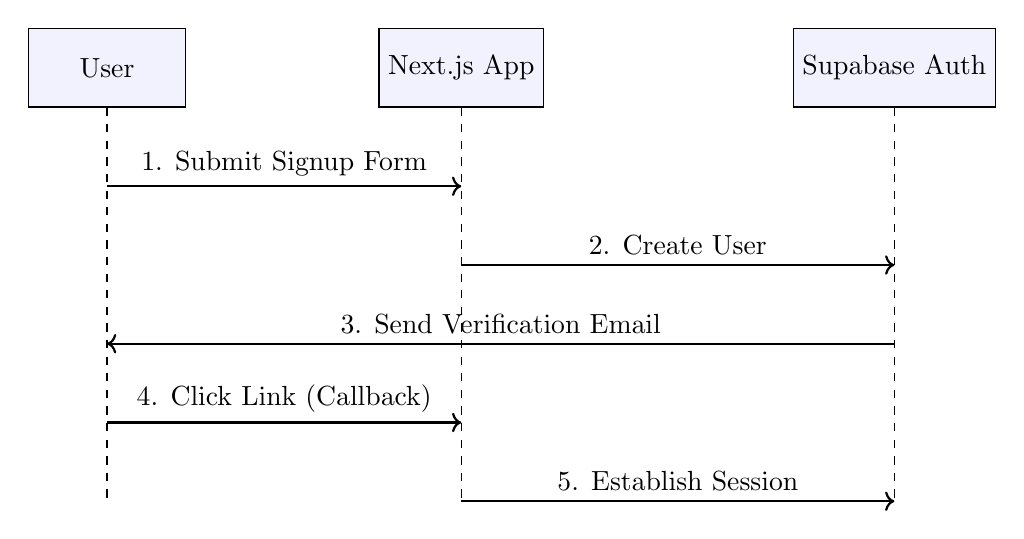
\begin{tikzpicture}[
        node distance=2.5cm,
        auto,
        box/.style={rectangle, draw, minimum width=2cm, minimum height=1cm, align=center, fill=blue!5},
        arrow/.style={->, thick}
    ]
    
    \node[box] (user) {User};
    \node[box, right of=user, xshift=2cm] (next) {Next.js App};
    \node[box, right of=next, xshift=3cm] (supa) {Supabase Auth};
    
    \draw[dashed] (user.south) -- +(0,-5cm);
    \draw[dashed] (next.south) -- +(0,-5cm);
    \draw[dashed] (supa.south) -- +(0,-5cm);
    
    \draw[arrow] ([yshift=-1cm]user.south) -- node[above] {1. Submit Signup Form} ([yshift=-1cm]next.south);
    \draw[arrow] ([yshift=-2cm]next.south) -- node[above] {2. Create User} ([yshift=-2cm]supa.south);
    \draw[arrow] ([yshift=-3cm]supa.south) -- node[above] {3. Send Verification Email} ([yshift=-3cm]user.south);
    \draw[arrow] ([yshift=-4cm]user.south) -- node[above] {4. Click Link (Callback)} ([yshift=-4cm]next.south);
    \draw[arrow] ([yshift=-5cm]next.south) -- node[above] {5. Establish Session} ([yshift=-5cm]supa.south);
    
    \end{tikzpicture}
    \caption{Authentication Sequence Diagram}
    \label{fig:auth_flow}
\end{figure}

\section{Key Portal Features}

\subsection{E-Commerce and Product Management}
The "Summit Gear" store allows users to browse climbing equipment and the tracker devices.
The system implements a standard e-commerce flow: Product Browsing $\rightarrow$ Cart $\rightarrow$ Checkout. Administrators can manage product listings, update stock levels, and process incoming orders via a protected admin dashboard.

\begin{figure}[htbp]
    \centering
    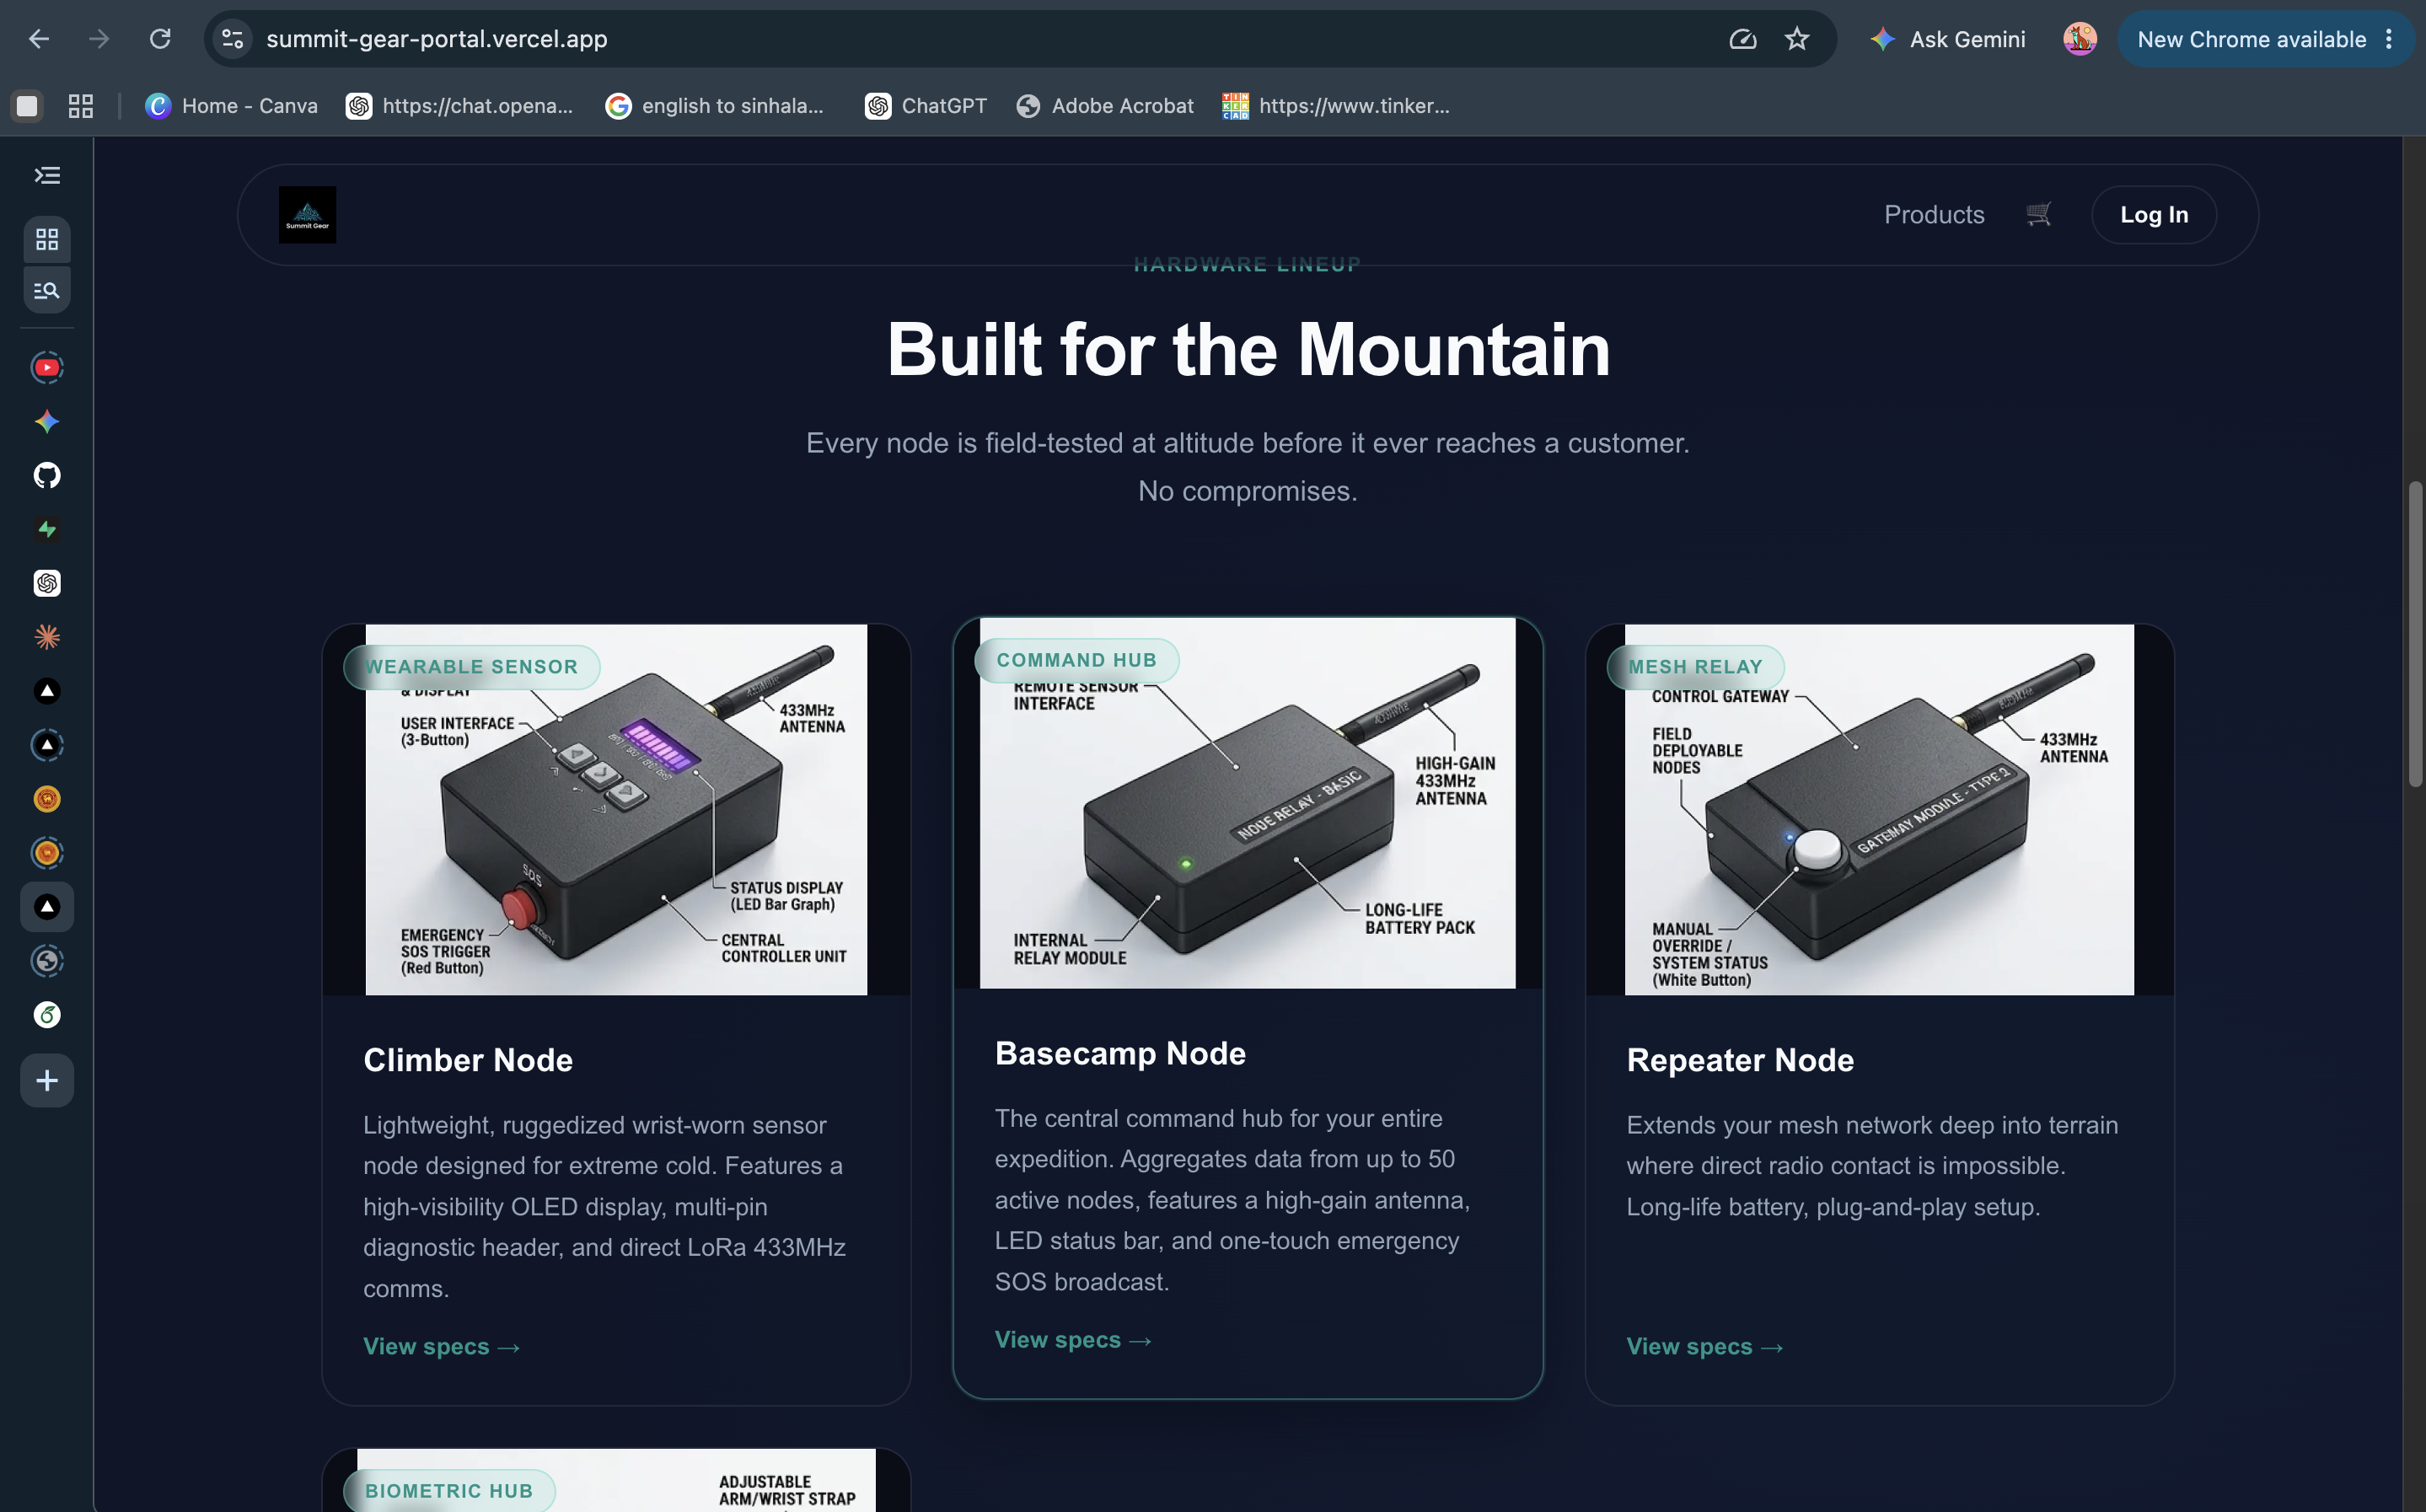
\includegraphics[width=0.9\textwidth]{portal_store.png}
    \caption{Summit Gear E-Commerce Interface}
    \label{fig:portal_store}
\end{figure}

\subsection{Device Registration Workflow}
When a user purchases a Climber Health Tracker, they must register the device on the portal using a unique serial number. 
This workflow links the physical device's MAC address and LoRa Node ID to the user's account in the PostgreSQL database. Row-Level Security (RLS) in Supabase ensures that users can only view and manage devices registered to their own account.

\subsection{Firmware Downloads}
The portal provides a secure section for registered users to download the latest OTA (Over-The-Air) firmware binaries. The Next.js backend verifies the user's session and device ownership before granting access to the firmware files stored in Supabase Storage.

\chapter{Database Design}
\label{ch:database_design}

The Summit Gear web portal and device management system rely on a robust, relational database architecture hosted on Supabase, a managed PostgreSQL platform. This chapter details the database schema, entity relationships, security policies, and the SQL statements used for initialization.

\section{Entity-Relationship Model}

The database schema is designed to handle e-commerce operations, user management, and IoT device registration. The core entities include users, products, orders, order items, devices, and firmware releases. Figure \ref{fig:er_diagram} illustrates the relationships between these entities.

\begin{figure}[htbp]
    \centering
    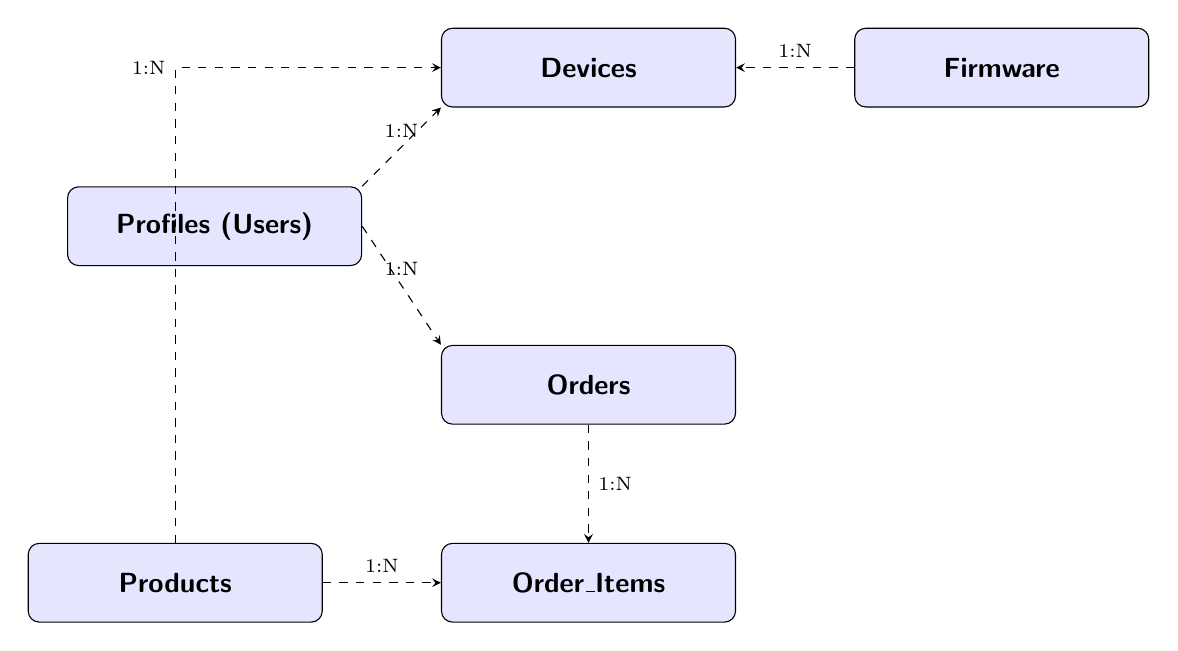
\begin{tikzpicture}[
        node distance=2.5cm and 3cm,
        every node/.style={font=\sffamily\small},
        entity/.style={draw, rectangle, rounded corners, fill=blue!10, text centered, text width=3.5cm, minimum height=1cm, font=\bfseries\sffamily},
        attribute/.style={draw, ellipse, fill=yellow!20, text centered, text width=2.5cm},
        relationship/.style={draw, diamond, aspect=2, fill=green!20, text centered, text width=2cm},
        line/.style={draw, -stealth}
    ]
        % Entities
        \node[entity] (users) {Profiles (Users)};
        \node[entity, below right=1cm and 1cm of users] (orders) {Orders};
        \node[entity, below=1.5cm of orders] (order_items) {Order\_Items};
        \node[entity, left=1.5cm of order_items] (products) {Products};
        \node[entity, above right=1cm and 1cm of users] (devices) {Devices};
        \node[entity, right=1.5cm of devices] (firmware) {Firmware};

        % Relationships
        \draw[line, dashed] (users.east) -- node[above, font=\scriptsize] {1:N} (orders.north west);
        \draw[line, dashed] (orders.south) -- node[right, font=\scriptsize] {1:N} (order_items.north);
        \draw[line, dashed] (products.east) -- node[above, font=\scriptsize] {1:N} (order_items.west);
        \draw[line, dashed] (users.north east) -- node[above, font=\scriptsize] {1:N} (devices.south west);
        \draw[line, dashed] (products.north) |- node[left, font=\scriptsize] {1:N} (devices.west);
        \draw[line, dashed] (firmware.west) -- node[above, font=\scriptsize] {1:N} (devices.east);
    \end{tikzpicture}
    \caption{Entity-Relationship Diagram of the Supabase PostgreSQL Schema.}
    \label{fig:er_diagram}
\end{figure}

\section{Table Definitions and SQL Schema}

The relational schema is implemented in PostgreSQL. The `profiles` table is automatically linked to Supabase's built-in authentication system.

\subsection{SQL Initialization Script}

\begin{lstlisting}[language=SQL, caption=PostgreSQL Schema Creation Script, label=lst:sql_schema]
-- Enable UUID extension
CREATE EXTENSION IF NOT EXISTS "uuid-ossp";

-- Profiles (extends Supabase Auth Users)
CREATE TABLE profiles (
    id UUID REFERENCES auth.users(id) PRIMARY KEY,
    email TEXT UNIQUE NOT NULL,
    full_name TEXT,
    role TEXT DEFAULT 'customer' CHECK (role IN ('customer', 'admin')),
    created_at TIMESTAMPTZ DEFAULT NOW()
);

-- Products
CREATE TABLE products (
    id UUID PRIMARY KEY DEFAULT uuid_generate_v4(),
    name TEXT NOT NULL,
    description TEXT,
    price DECIMAL(10, 2) NOT NULL,
    image_url TEXT,
    category TEXT,
    stock INTEGER DEFAULT 0,
    created_at TIMESTAMPTZ DEFAULT NOW()
);

-- Orders
CREATE TABLE orders (
    id UUID PRIMARY KEY DEFAULT uuid_generate_v4(),
    user_id UUID REFERENCES profiles(id) NOT NULL,
    status TEXT DEFAULT 'pending',
    total DECIMAL(10, 2) NOT NULL,
    shipping_address TEXT NOT NULL,
    created_at TIMESTAMPTZ DEFAULT NOW()
);

-- Order Items
CREATE TABLE order_items (
    id UUID PRIMARY KEY DEFAULT uuid_generate_v4(),
    order_id UUID REFERENCES orders(id) ON DELETE CASCADE,
    product_id UUID REFERENCES products(id),
    quantity INTEGER NOT NULL CHECK (quantity > 0),
    price DECIMAL(10, 2) NOT NULL
);

-- Firmware
CREATE TABLE firmware (
    id UUID PRIMARY KEY DEFAULT uuid_generate_v4(),
    version TEXT NOT NULL,
    device_type TEXT NOT NULL,
    download_url TEXT NOT NULL,
    release_notes TEXT,
    created_at TIMESTAMPTZ DEFAULT NOW()
);

-- Devices
CREATE TABLE devices (
    id UUID PRIMARY KEY DEFAULT uuid_generate_v4(),
    serial_number TEXT UNIQUE NOT NULL,
    user_id UUID REFERENCES profiles(id),
    product_id UUID REFERENCES products(id),
    firmware_version TEXT,
    registered_at TIMESTAMPTZ DEFAULT NOW()
);
\end{lstlisting}

\section{Row-Level Security (RLS) Policies}

To ensure data privacy and security, Supabase's Row-Level Security (RLS) is heavily utilized. RLS ensures that users can only access or modify data that belongs to them, while administrators retain full access.

\begin{infobox}
Row-Level Security is a PostgreSQL feature that restricts which rows are returned by normal queries, or are permitted for data modification commands, based on the user executing the query.
\end{infobox}

\subsection{Profiles Policy}
Users can only view and update their own profiles.
\begin{lstlisting}[language=SQL]
ALTER TABLE profiles ENABLE ROW LEVEL SECURITY;
CREATE POLICY "Users can view own profile" ON profiles
    FOR SELECT USING (auth.uid() = id);
CREATE POLICY "Users can update own profile" ON profiles
    FOR UPDATE USING (auth.uid() = id);
\end{lstlisting}

\subsection{Orders and Devices Policy}
Customers can only view their own orders and registered devices.
\begin{lstlisting}[language=SQL]
-- Orders
ALTER TABLE orders ENABLE ROW LEVEL SECURITY;
CREATE POLICY "Users can view own orders" ON orders
    FOR SELECT USING (auth.uid() = user_id);

-- Devices
ALTER TABLE devices ENABLE ROW LEVEL SECURITY;
CREATE POLICY "Users can view own devices" ON devices
    FOR SELECT USING (auth.uid() = user_id);
\end{lstlisting}

\subsection{Public Access Policies}
The \texttt{products} and \texttt{firmware} tables are publicly readable, allowing unauthenticated users to browse the catalog and devices to fetch firmware updates without complex authentication handshakes.

\begin{lstlisting}[language=SQL]
ALTER TABLE products ENABLE ROW LEVEL SECURITY;
CREATE POLICY "Products are publicly visible" ON products
    FOR SELECT USING (true);

ALTER TABLE firmware ENABLE ROW LEVEL SECURITY;
CREATE POLICY "Firmware is publicly visible" ON firmware
    FOR SELECT USING (true);
\end{lstlisting}

\chapter{Testing \& Validation}
\label{ch:testing}

Rigorous testing was conducted to ensure the reliability, accuracy, and robust performance of the Mountain Climber Health \& GPS Tracker system under simulated field conditions. This chapter presents the methodologies and results of various hardware and software tests.

\section{LoRa Range Testing}
\label{sec:lora_range}

Given the critical nature of communication in remote areas, the SX1278 LoRa modules were tested extensively for range and signal integrity under different spreading factors (SF) and line-of-sight (LOS) conditions.

\begin{infobox}
Testing was conducted at 433MHz with a bandwidth of 125kHz and a coding rate of 4/5. Transmission power was set to 20 dBm.
\end{infobox}

\subsection{Test Methodology}
Two nodes were utilized: a transmitter periodically sending 50-byte packets and a receiver logging the Received Signal Strength Indicator (RSSI) and Packet Delivery Ratio (PDR). Tests were performed in an open field (LOS) and a moderately wooded suburban area (Non-LOS).

\subsection{Results}

\begin{table}[htbp]
    \centering
    \caption{LoRa Range Testing Results (Transmitter Power: 20 dBm, BW: 125kHz)}
    \label{tab:lora_results}
    \resizebox{\textwidth}{!}{
    \begin{tabular}{llccc}
        \toprule
        \textbf{Environment} & \textbf{Spreading Factor} & \textbf{Distance (km)} & \textbf{Avg RSSI (dBm)} & \textbf{Packet Loss (\%)} \\
        \midrule
        Line-of-Sight (LOS)  & SF7  & 1.5 & -95  & 0.0 \\
        Line-of-Sight (LOS)  & SF7  & 3.0 & -108 & 2.1 \\
        Line-of-Sight (LOS)  & SF10 & 5.0 & -115 & 1.5 \\
        Non-LOS (Wooded)     & SF7  & 0.5 & -102 & 4.2 \\
        Non-LOS (Wooded)     & SF7  & 1.2 & -118 & 22.5 \\
        Non-LOS (Wooded)     & SF10 & 1.5 & -112 & 3.0 \\
        Non-LOS (Wooded)     & SF12 & 2.5 & -120 & 8.5 \\
        \bottomrule
    \end{tabular}
    }
\end{table}

The results in Table \ref{tab:lora_results} indicate that while SF7 provides adequate LOS range, utilizing higher spreading factors like SF10 or SF12 is crucial for maintaining low packet loss in non-LOS mountainous environments, albeit at the cost of lower data rates.

\begin{figure}[htbp]
    \centering
    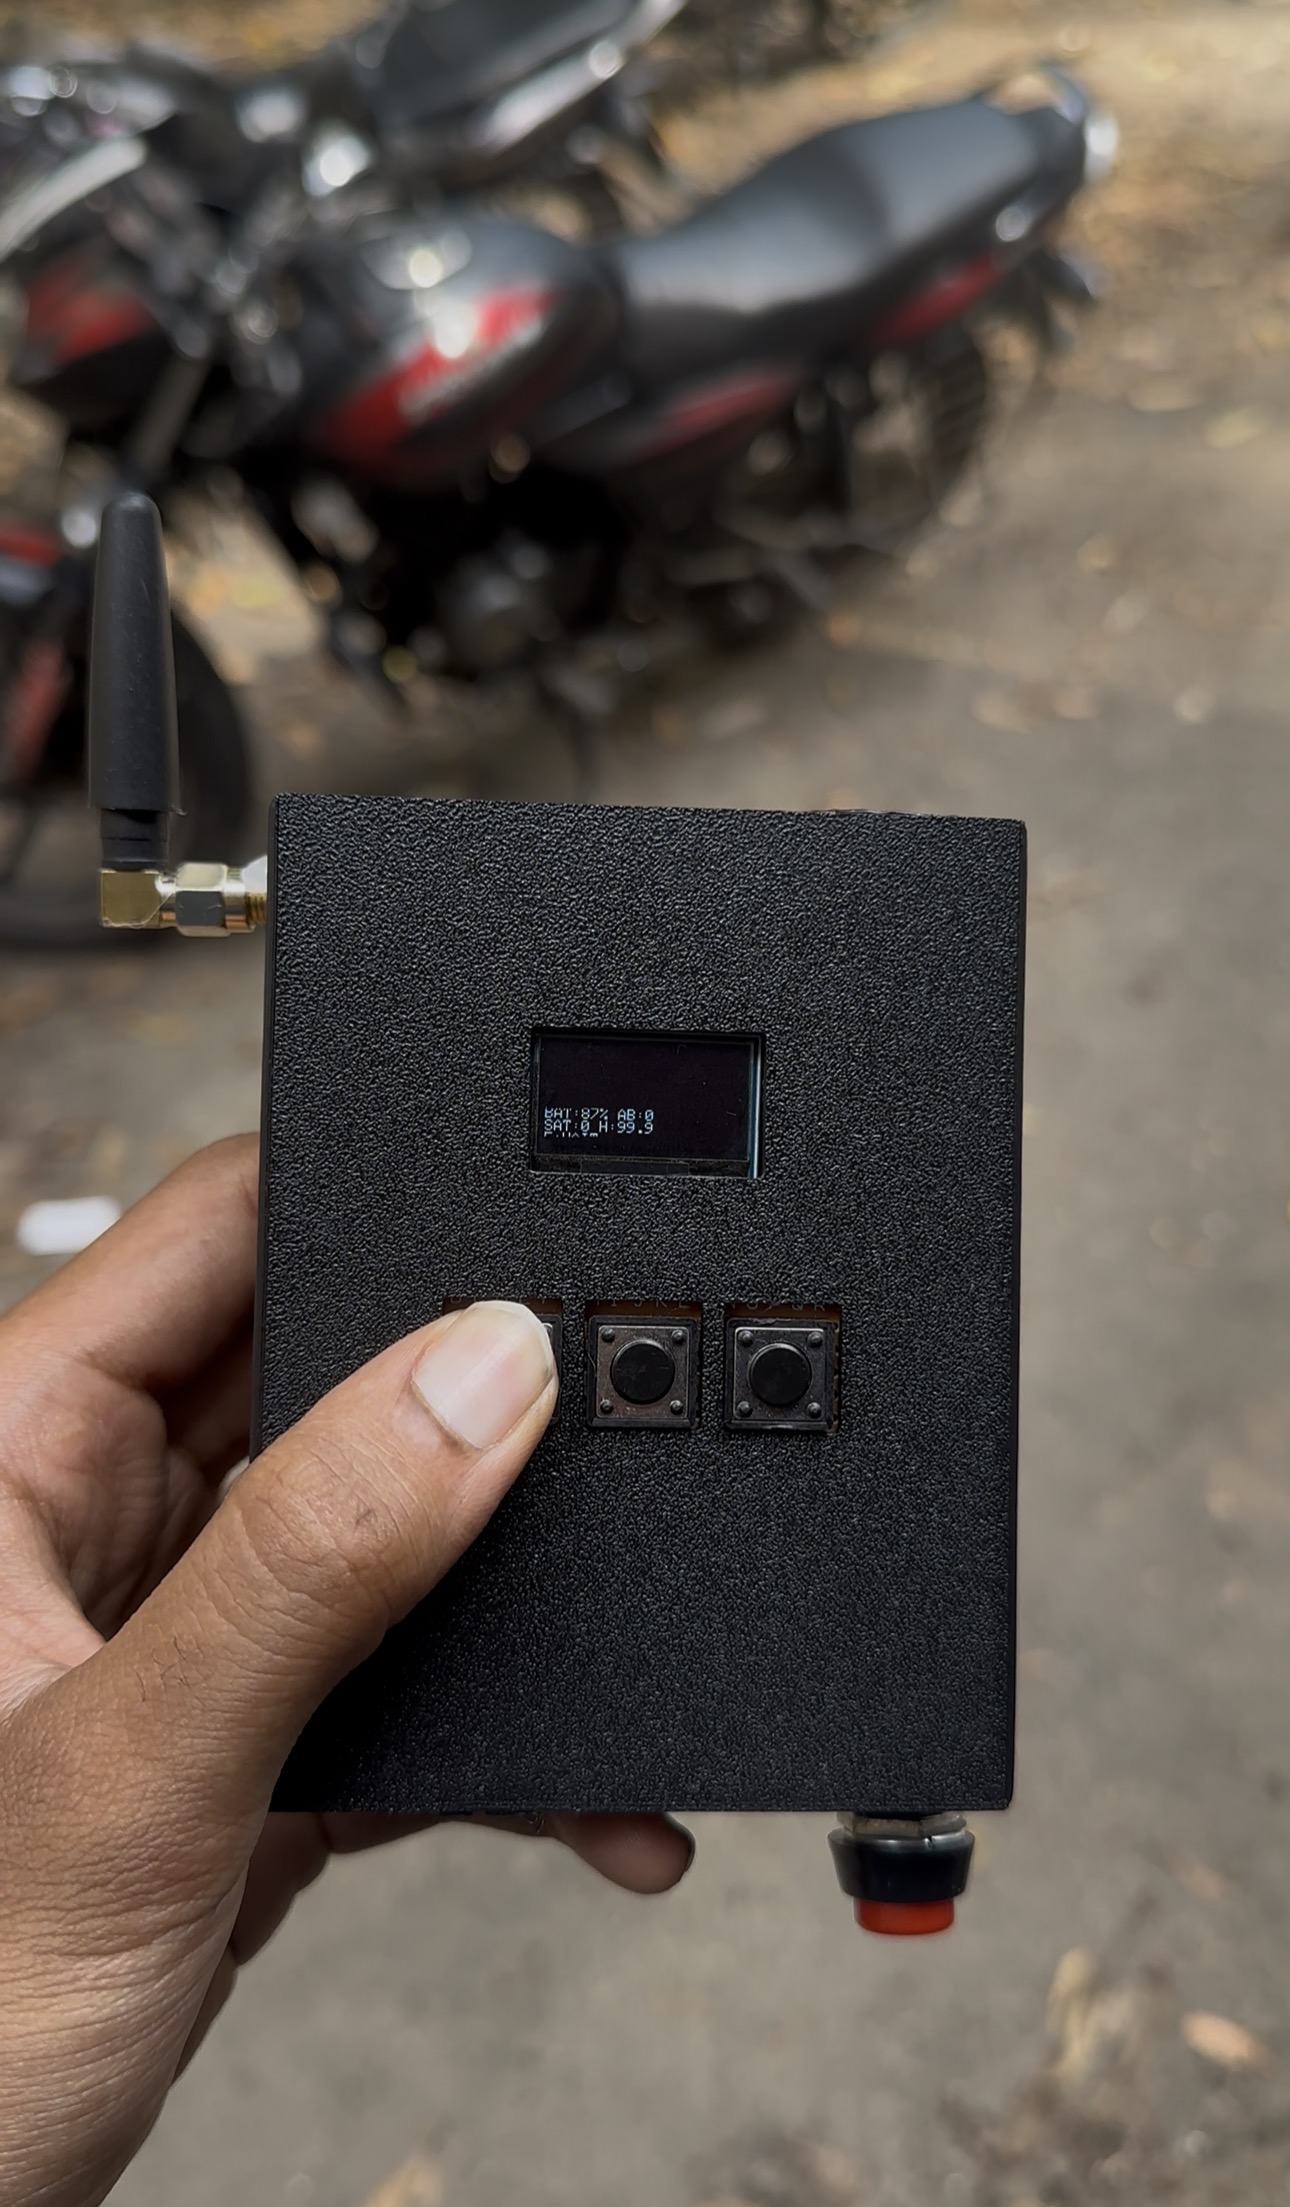
\includegraphics[width=0.8\textwidth]{lora_test_setup.png}
    \caption{LoRa Range Testing Setup in Field Conditions}
    \label{fig:lora_test_setup}
\end{figure}

\section{Sensor Accuracy Validation}
\label{sec:sensor_testing}

\subsection{MAX30102 Health Sensor}
The MAX30102 sensor's heart rate (BPM) and blood oxygen saturation (SpO2) readings were validated against a medical-grade finger pulse oximeter (ChoiceMMed MD300C2). 

\begin{table}[htbp]
    \centering
    \caption{MAX30102 Accuracy Comparison (Resting State, N=50 samples)}
    \label{tab:max_accuracy}
    \resizebox{\textwidth}{!}{
    \begin{tabular}{lccc}
        \toprule
        \textbf{Metric} & \textbf{Reference Device (Avg)} & \textbf{MAX30102 (Avg)} & \textbf{Mean Absolute Error} \\
        \midrule
        Heart Rate (BPM) & 72.4 & 73.1 & 1.8 BPM \\
        SpO2 (\%)        & 98.2 & 97.5 & 0.9 \% \\
        \bottomrule
    \end{tabular}
    }
\end{table}

\begin{warningbox}
While resting accuracy is within acceptable margins, vigorous wrist movement introduces motion artifacts, occasionally resulting in SpO2 reading dropouts.
\end{warningbox}

\subsection{NEO-6M GPS Module}
GPS accuracy was tested by placing the module at known surveyed coordinates. The module achieved a typical horizontal position error of 2.5 to 4 meters under clear skies (Time-To-First-Fix: $\sim$35 seconds from cold start).

\section{BLE Connection Reliability}
\label{sec:ble_testing}

The BLE link between the Wristband/Climber Main device and the Flutter mobile application was tested for connection stability and automatic reconnection.

\begin{itemize}
    \item \textbf{Connection Time:} Average 1.2 seconds to establish connection and discover GATT services.
    \item \textbf{Range:} Reliable connection maintained up to 8 meters indoors and 15 meters outdoors.
    \item \textbf{Reconnection Behavior:} When the connection drops due to distance, the Flutter app successfully reconnects automatically within 3 seconds of re-entering the range.
\end{itemize}

\section{System Integration Testing}
\label{sec:integration_testing}

An end-to-end integration test was conducted to verify the complete data pipeline from the climber to the base camp dashboard.

\textbf{Test Scenario: SOS Emergency Trigger}
\begin{enumerate}
    \item \textbf{Trigger:} Climber presses the physical SOS button on the Main Device.
    \item \textbf{Local Action:} Device buzzer activates, RGB LED turns red, and the Flutter app immediately displays a local emergency warning via BLE.
    \item \textbf{LoRa Transmission:} An SOS packet (Type 0x01) containing current GPS coordinates is broadcast via LoRa.
    \item \textbf{Relay:} The intermediate Repeater node successfully receives, validates the CRC, and re-broadcasts the packet.
    \item \textbf{Reception:} Base Camp unit receives the packet, outputs JSON over serial to the connected laptop.
    \item \textbf{Dashboard Alert:} The Flask dashboard parses the JSON, plays a loud audio alarm, flashes the screen red, and updates the climber's marker on the real-time map to indicate an emergency state.
\end{enumerate}

\textbf{Result:} The entire pipeline, from button press to dashboard alarm, consistently executed in under 1.5 seconds.

\chapter{Budget \& Bill of Materials}
\label{ch:budget}

This chapter details the financial planning for the Mountain Climber Health \& GPS Tracker. The budget is divided into hardware component costs (Bill of Materials) and general development and deployment costs. All prices are estimated in Sri Lankan Rupees (LKR) based on local electronics suppliers at the time of development.

\section{Device Bill of Materials (BOM)}

The system consists of three distinct hardware units. Table \ref{tab:bom} outlines the components required for a single Climber Main Device, which is the most complex unit in the system.

\begin{table}[htbp]
    \centering
    \caption{Bill of Materials for a Single Climber Main Device}
    \label{tab:bom}
    \resizebox{\textwidth}{!}{
    \begin{tabular}{llccc}
        \toprule
        \textbf{Component} & \textbf{Specification} & \textbf{Qty} & \textbf{Unit Cost (LKR)} & \textbf{Total (LKR)} \\
        \midrule
        Microcontroller & ESP32 DevKit V1 & 1 & 2,500 & 2,500 \\
        Health Sensor & MAX30102 Pulse Oximeter & 1 & 800 & 800 \\
        GPS Module & Ublox NEO-6M & 1 & 1,500 & 1,500 \\
        LoRa Transceiver & SX1278 (433MHz) & 1 & 1,200 & 1,200 \\
        Power Supply & 18650 Li-ion Battery (3.7V) & 1 & 600 & 600 \\
        Charging Module & TP4056 Battery Charger & 1 & 250 & 250 \\
        Enclosure & Custom 3D Printed / ABS & 1 & 500 & 500 \\
        Miscellaneous & PCBs, Wires, Connectors, LEDs & 1 & 800 & 800 \\
        \midrule
        \multicolumn{4}{r}{\textbf{Total Cost per Climber Device}} & \textbf{8,150} \\
        \bottomrule
    \end{tabular}
    }
\end{table}

\begin{infobox}
The Wristband, Repeater, and Base Camp units utilize subsets of these components. For example, a Repeater only requires an ESP32, SX1278, battery, and enclosure, bringing its unit cost down to approximately LKR 5,650.
\end{infobox}

\section{Total Hardware System Cost}

For a standard expedition setup, the system is designed to support multiple climbers and require relay nodes depending on the terrain. Table \ref{tab:system_cost} calculates the cost for a typical base configuration consisting of two climbers, one repeater, and one base camp unit.

\begin{table}[htbp]
    \centering
    \caption{Hardware Cost for a Standard Expedition Setup}
    \label{tab:system_cost}
    \resizebox{\textwidth}{!}{
    \begin{tabular}{lccc}
        \toprule
        \textbf{Unit Type} & \textbf{Estimated Unit Cost (LKR)} & \textbf{Quantity} & \textbf{Total (LKR)} \\
        \midrule
        Climber Main Device & 8,150 & 2 & 16,300 \\
        Wristband Device (BLE) & 4,500 & 2 & 9,000 \\
        Repeater Node & 5,650 & 1 & 5,650 \\
        Base Camp Unit & 5,200 & 1 & 5,200 \\
        \midrule
        \multicolumn{3}{r}{\textbf{Total Hardware System Cost}} & \textbf{36,150} \\
        \bottomrule
    \end{tabular}
    }
\end{table}

\section{Software and Development Costs}

While the system heavily utilizes open-source software (Flutter, Python, PostgreSQL), there are infrastructural costs associated with hosting the web portal, database, and domain names.

\begin{table}[htbp]
    \centering
    \caption{Development and Infrastructure Costs}
    \label{tab:dev_cost}
    \resizebox{\textwidth}{!}{
    \begin{tabular}{llc}
        \toprule
        \textbf{Item} & \textbf{Description} & \textbf{Cost (LKR)} \\
        \midrule
        Domain Name & summitgear.com (Annual) & 4,500 \\
        Web Hosting (Vercel) & Next.js frontend hosting & Free Tier \\
        Database Hosting (Supabase) & PostgreSQL, Auth, Storage & Free Tier \\
        Development Tools & Soldering supplies, multimeters & 3,500 \\
        Prototyping Waste & Damaged/burnt components during R\&D & 2,500 \\
        \midrule
        \multicolumn{2}{r}{\textbf{Total Development Costs}} & \textbf{10,500} \\
        \bottomrule
    \end{tabular}
    }
\end{table}

\section{Budget Summary}

The grand total for deploying the prototype system, including a standard hardware configuration and initial infrastructure setup, is calculated as follows:

\begin{table}[htbp]
    \centering
    \caption{Grand Total Budget Summary}
    \label{tab:grand_total}
    \begin{tabular}{lr}
        \toprule
        \textbf{Category} & \textbf{Amount (LKR)} \\
        \midrule
        Hardware System Cost & 36,150 \\
        Development \& Infrastructure Costs & 10,500 \\
        \midrule
        Contingency Fund (10\%) & 4,665 \\
        \midrule
        \textbf{Grand Total Estimate} & \textbf{51,315} \\
        \bottomrule
    \end{tabular}
\end{table}

\chapter{Limitations \& Future Work}
\label{ch:limitations}

While the current prototype of the Mountain Climber Health \& GPS Tracker successfully demonstrates the core functionalities of off-grid safety monitoring, several limitations were identified during development and testing. This chapter outlines these constraints and proposes future enhancements for a production-ready system.

\section{Known Limitations}

\begin{itemize}
    \item \textbf{GPS Accuracy in Dense Canopy:} The Ublox NEO-6M module struggles to acquire a fast and accurate satellite fix under dense forest canopies or deep ravines, potentially delaying location updates during an emergency.
    \item \textbf{LoRa Line-of-Sight Dependency:} While 433MHz penetrates vegetation better than 2.4GHz, extreme geological features (steep valleys, massive rock faces) severely attenuate the signal, necessitating careful, manual placement of Repeater nodes.
    \item \textbf{Motion Artifacts on MAX30102:} The optical pulse oximetry sensor is highly sensitive to ambient light and movement. Vigorous climbing motions can introduce noise, leading to temporarily inaccurate heart rate or SpO2 readings.
    \item \textbf{Single-Channel LoRa Limitations:} The system currently uses a single LoRa channel and spreading factor. It lacks frequency hopping or adaptive data rates, meaning network collisions can occur if many devices transmit simultaneously in a dense deployment.
    \item \textbf{Battery Constraints:} Constantly polling GPS and listening on the LoRa radio draws significant current. Without power optimization, the 18650 battery life is limited to approximately 18-24 hours of continuous operation.
\end{itemize}

\section{Future Improvements}

To address these limitations and commercialize the system, the following future works are proposed:

\subsection{Hardware Enhancements}
\begin{itemize}
    \item \textbf{Multi-channel LoRa Gateway:} Upgrading the Base Camp unit to a multi-channel LoRaWAN gateway (e.g., using SX1302) to handle hundreds of concurrent nodes and implement Adaptive Data Rate (ADR) protocols.
    \item \textbf{Solar Energy Harvesting:} Integrating small, flexible solar panels into the device enclosures or backpacks to trickle-charge the lithium batteries, significantly extending deployment life.
    \item \textbf{Satellite Communication Fallback:} Integrating an Iridium or Swarm satellite modem for extreme emergencies when the climber falls completely outside the LoRa mesh network range.
    \item \textbf{IP67 Waterproofing:} Designing injection-molded enclosures with silicone gaskets to achieve true IP67 weather resistance for harsh alpine environments.
\end{itemize}

\subsection{Software \& System Enhancements}
\begin{itemize}
    \item \textbf{Mesh Routing Protocol:} Implementing an intelligent, self-healing mesh routing protocol (like Reticulum or Meshtastic's underlying logic) to replace the current static repeater logic.
    \item \textbf{Machine Learning Health Predictions:} Developing ML models that run on the dashboard to analyze vitals trends over time, predicting altitude sickness or exhaustion before acute symptoms appear.
    \item \textbf{Cloud Dashboard Sync:} Developing a mechanism for the local Base Camp dashboard to opportunistically sync its data to the Next.js cloud portal whenever an intermittent internet connection (e.g., via Starlink or cellular) is available.
\end{itemize}


% ── Appendices ──
\appendix
\chapter{Pin Configuration Tables}
\label{app:pin_configs}

This appendix provides the complete General Purpose Input/Output (GPIO) mapping for all microcontrollers utilized in the Mountain Climber Health \& GPS Tracker system.

\section{Climber Main Device (ESP32)}
\begin{table}[htbp]
    \centering
    \resizebox{\textwidth}{!}{
    \begin{tabular}{clll}
        \toprule
        \textbf{GPIO Number} & \textbf{Connected To} & \textbf{Function} & \textbf{Protocol} \\
        \midrule
        GPIO 5  & SX1278 NSS & LoRa Chip Select & SPI \\
        GPIO 18 & SX1278 SCK & SPI Clock & SPI \\
        GPIO 19 & SX1278 MISO & SPI Master In Slave Out & SPI \\
        GPIO 23 & SX1278 MOSI & SPI Master Out Slave In & SPI \\
        GPIO 14 & SX1278 RST & LoRa Reset & Digital Out \\
        GPIO 26 & SX1278 DIO0 & LoRa Interrupt & Digital In \\
        GPIO 21 & MAX30102 SDA & I2C Data & I2C \\
        GPIO 22 & MAX30102 SCL & I2C Clock & I2C \\
        GPIO 16 & NEO-6M TX & GPS Data Transmit & UART2 RX \\
        GPIO 17 & NEO-6M RX & GPS Data Receive & UART2 TX \\
        GPIO 4  & Active Buzzer & Audio Alarm & Digital Out/PWM \\
        GPIO 25 & RGB LED Red & Visual Status Indicator & Digital Out \\
        GPIO 33 & RGB LED Green & Visual Status Indicator & Digital Out \\
        GPIO 32 & RGB LED Blue & Visual Status Indicator & Digital Out \\
        GPIO 13 & Tactile Push Button & SOS Trigger & Digital In (Pull-up) \\
        \bottomrule
    \end{tabular}
    }
\end{table}

\section{Wristband Device (ESP32-C3 / PICO)}
\begin{table}[htbp]
    \centering
    \resizebox{\textwidth}{!}{
    \begin{tabular}{clll}
        \toprule
        \textbf{GPIO Number} & \textbf{Connected To} & \textbf{Function} & \textbf{Protocol} \\
        \midrule
        GPIO 21 & MAX30102 SDA & I2C Data & I2C \\
        GPIO 22 & MAX30102 SCL & I2C Clock & I2C \\
        GPIO 9  & Battery Voltage ADC & Power Monitoring & Analog In \\
        GPIO 4  & Haptic Motor & Vibration Alert & Digital Out/PWM \\
        GPIO 5  & System LED & Status Indicator & Digital Out \\
        \bottomrule
    \end{tabular}
    }
\end{table}

\section{Repeater Node (ESP32)}
\begin{table}[htbp]
    \centering
    \begin{tabular}{clll}
        \toprule
        \textbf{GPIO Number} & \textbf{Connected To} & \textbf{Function} & \textbf{Protocol} \\
        \midrule
        GPIO 5  & SX1278 NSS & LoRa Chip Select & SPI \\
        GPIO 18 & SX1278 SCK & SPI Clock & SPI \\
        GPIO 19 & SX1278 MISO & SPI Master In Slave Out & SPI \\
        GPIO 23 & SX1278 MOSI & SPI Master Out Slave In & SPI \\
        GPIO 14 & SX1278 RST & LoRa Reset & Digital Out \\
        GPIO 26 & SX1278 DIO0 & LoRa Interrupt & Digital In \\
        GPIO 2  & Status LED & Node Active Indicator & Digital Out \\
        \bottomrule
    \end{tabular}
\end{table}

\section{Base Camp Unit (ESP32)}
\begin{table}[htbp]
    \centering
    \begin{tabular}{clll}
        \toprule
        \textbf{GPIO Number} & \textbf{Connected To} & \textbf{Function} & \textbf{Protocol} \\
        \midrule
        GPIO 5  & SX1278 NSS & LoRa Chip Select & SPI \\
        GPIO 18 & SX1278 SCK & SPI Clock & SPI \\
        GPIO 19 & SX1278 MISO & SPI Master In Slave Out & SPI \\
        GPIO 23 & SX1278 MOSI & SPI Master Out Slave In & SPI \\
        GPIO 14 & SX1278 RST & LoRa Reset & Digital Out \\
        GPIO 26 & SX1278 DIO0 & LoRa Interrupt & Digital In \\
        TX0 (GPIO 1)& PC USB Serial & JSON Data to Dashboard & UART0 \\
        RX0 (GPIO 3)& PC USB Serial & Commands from Dashboard& UART0 \\
        \bottomrule
    \end{tabular}
\end{table}

\chapter{LoRa Packet Format Specification}
\label{app:packet_format}

To optimize airtime and maximize the range of the LoRa transmissions, a custom, lightweight binary packet protocol is utilized instead of transmitting verbose string formats. This appendix details the byte-level structure.

\section{General Packet Structure}

Every transmission adheres to a standard header format followed by a variable-length payload.

\begin{figure}[htbp]
    \centering
    \resizebox{\textwidth}{!}{
    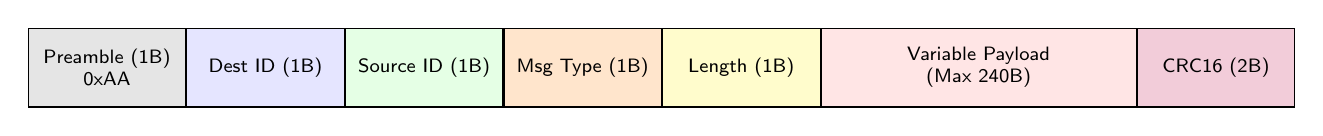
\begin{tikzpicture}[
        byte/.style={draw, rectangle, minimum height=1cm, align=center, font=\sffamily\scriptsize},
        node distance=0cm
    ]
        \node[byte, minimum width=2cm, fill=gray!20] (preamble) {Preamble (1B)\\0xAA};
        \node[byte, minimum width=2cm, right=of preamble, fill=blue!10] (dest) {Dest ID (1B)};
        \node[byte, minimum width=2cm, right=of dest, fill=green!10] (source) {Source ID (1B)};
        \node[byte, minimum width=2cm, right=of source, fill=orange!20] (type) {Msg Type (1B)};
        \node[byte, minimum width=2cm, right=of type, fill=yellow!20] (len) {Length (1B)};
        \node[byte, minimum width=4cm, right=of len, fill=red!10] (payload) {Variable Payload\\(Max 240B)};
        \node[byte, minimum width=2cm, right=of payload, fill=purple!20] (crc) {CRC16 (2B)};
    \end{tikzpicture}
    }
    \caption{Binary LoRa Packet Structure}
    \label{fig:packet-structure}
\end{figure}

\section{Message Types and Payload Definitions}

The \texttt{Msg Type} byte dictates how the receiver should parse the payload.

\subsection{0x01: SOS Alert}
Transmitted when a climber triggers an emergency.
\begin{itemize}
    \item \textbf{Payload Length:} 8 bytes
    \item \textbf{Structure:} [Latitude (4B Float)] [Longitude (4B Float)]
\end{itemize}

\subsection{0x02: Routine GPS Update}
Periodic location update.
\begin{itemize}
    \item \textbf{Payload Length:} 8 bytes
    \item \textbf{Structure:} [Latitude (4B Float)] [Longitude (4B Float)]
\end{itemize}

\subsection{0x03: Health Vitals}
Periodic or on-demand health data.
\begin{itemize}
    \item \textbf{Payload Length:} 3 bytes
    \item \textbf{Structure:} [Heart Rate BPM (1B Uint)] [SpO2 \% (1B Uint)] [Temperature C (1B Int)]
\end{itemize}

\subsection{0x04: Text Message}
Two-way chat messages.
\begin{itemize}
    \item \textbf{Payload Length:} 1 to 240 bytes
    \item \textbf{Structure:} [ASCII Text String]
\end{itemize}

\section{Example Hex Dumps}

\textbf{Example 1: Health Vitals Update}
Climber 0x05 sends health data to Base Camp 0x00. HR=85, SpO2=98, Temp=24.
\begin{verbatim}
AA 00 05 03 03 55 62 18 [CRC_H] [CRC_L]
\end{verbatim}
\textit{Breakdown: AA (Preamble), 00 (Dest Base), 05 (Source Climber), 03 (MsgType Health), 03 (Len 3), 55 (85 BPM), 62 (98\%), 18 (24C).}

\textbf{Example 2: SOS Alert}
Climber 0x02 triggers SOS with coordinates 7.2906, 80.6337.
\begin{verbatim}
AA 00 02 01 08 40 E9 4B 38 42 A1 44 80 [CRC_H] [CRC_L]
\end{verbatim}
\textit{Breakdown: The 8-byte payload represents the two 32-bit IEEE 754 floats for Lat and Lng.}

\chapter{API Reference}
\label{app:api_ref}

This appendix documents the key Application Programming Interfaces (APIs) used for communication between the Flask Base Camp Dashboard and the Next.js Supabase web portal.

\section{Base Camp Dashboard (Flask REST API)}

The Python Flask dashboard exposes a local API that the desktop UI interacts with to retrieve serial data and send commands.

\subsection{\texttt{GET /}}
Renders the main dashboard HTML interface.
\begin{itemize}
    \item \textbf{Authentication:} None (Localhost only)
    \item \textbf{Response:} HTML page.
\end{itemize}

\subsection{\texttt{GET /get\_data}}
Polls the latest telemetry data received from the serial port.
\begin{itemize}
    \item \textbf{Authentication:} None
    \item \textbf{Response:} JSON Array of climber objects.
\end{itemize}
\begin{lstlisting}
{
  "climbers": [
    {
      "id": 5,
      "lat": 7.2906,
      "lng": 80.6337,
      "hr": 85,
      "spo2": 98,
      "status": "normal",
      "last_seen": "2024-05-20T10:30:00Z"
    }
  ]
}
\end{lstlisting}

\subsection{\texttt{POST /send\_message}}
Queues a text message to be transmitted via LoRa to a specific climber.
\begin{itemize}
    \item \textbf{Request Body (JSON):}
    \begin{lstlisting}
    {
      "dest_id": 5,
      "message": "Weather deteriorating. Return to base."
    }
    \end{lstlisting}
    \item \textbf{Response:} HTTP 200 OK
\end{itemize}

\subsection{\texttt{GET /export\_csv}}
Triggers a download of all logged telemetry data for post-expedition analysis.
\begin{itemize}
    \item \textbf{Response:} \texttt{text/csv} file download.
\end{itemize}

\section{Summit Gear Web Portal (Next.js Server Actions)}

The Next.js portal utilizes Server Actions for interacting with the Supabase database. These act as secure, server-side API endpoints.

\subsection{\texttt{registerDevice(serialNum, userId)}}
Registers a new physical device to a user's account.
\begin{itemize}
    \item \textbf{Auth Required:} Yes (Valid session JWT)
    \item \textbf{Response:} Success boolean or error message.
\end{itemize}

\subsection{\texttt{createOrder(cart: CartItem[], userId: string)}}
Processes an e-commerce checkout.
\begin{itemize}
    \item \textbf{Auth Required:} Yes
    \item \textbf{Response:} Order UUID string.
\end{itemize}

\subsection{\texttt{getProducts(category?: string)}}
Fetches the catalog of available gear and devices.
\begin{itemize}
    \item \textbf{Auth Required:} No
    \item \textbf{Response:} Array of Product objects.
\end{itemize}

\subsection{\texttt{uploadFirmware(file: FormData, version: string)}}
Admin-only endpoint to upload a new OTA firmware binary.
\begin{itemize}
    \item \textbf{Auth Required:} Yes (Role must be 'admin')
    \item \textbf{Response:} Download URL of the uploaded asset in Supabase Storage.
\end{itemize}


\end{document}
